\documentclass[compress]{beamer}
\usepackage{ifthen,verbatim,hyperref}

\newcommand{\isnote}{}
\xdefinecolor{lightyellow}{rgb}{1.,1.,0.25}
\xdefinecolor{darkblue}{rgb}{0.1,0.1,0.7}
\xdefinecolor{darkred}{rgb}{0.9,0.,0.}
\xdefinecolor{lightblue}{rgb}{0.2,0.6,0.6}

%% Uncomment this to get annotations
%% \def\notes{\addtocounter{page}{-1}
%%            \renewcommand{\isnote}{*}
%% 	   \beamertemplateshadingbackground{lightyellow}{white}
%%            \begin{frame}
%%            \frametitle{Notes for the previous page (page \insertpagenumber)}
%%            \itemize}
%% \def\endnotes{\enditemize
%% 	      \end{frame}
%%               \beamertemplateshadingbackground{white}{white}
%%               \renewcommand{\isnote}{}}

%% Uncomment this to not get annotations
\def\notes{\comment}
\def\endnotes{\endcomment}

\setbeamertemplate{navigation symbols}{}
\setbeamertemplate{headline}{\mbox{ } \hfill
\begin{minipage}{5.5 cm}
\vspace{-0.75 cm} \small
\end{minipage} \hfill
\begin{minipage}{4.5 cm}
\vspace{-0.75 cm} \small
\begin{flushright}
\ifthenelse{\equal{\insertpagenumber}{0}}{}{Jim Pivarski \hspace{0.2 cm} \insertpagenumber\isnote/\pageref{numpages}}
\end{flushright}
\end{minipage}\mbox{\hspace{0.2 cm}}\includegraphics[height=1 cm]{../cmslogo} \hspace{0.1 cm} \includegraphics[height=1 cm]{../tamulogo} \hspace{0.01 cm} \vspace{-1.05 cm}}

\begin{document}
%% \begin{frame}
%% \vfill
%% \begin{center}
%% \textcolor{darkblue}{\LARGE Toward Precision Muon Tracking: \\ \Large \vspace{0.2 cm} Understanding the CMS Magnetic Field \\ \vspace{0.2 cm} and Other Effects in CRAFT}

%% \vfill
%% \begin{columns}
%% \column{0.3\linewidth}
%% \begin{center}
%% \large
%% \textcolor{darkblue}{Jim Pivarski}
%% \end{center}
%% \end{columns}

%% \begin{columns}
%% \column{0.3\linewidth}
%% \begin{center}
%% \scriptsize
%% {\it Texas A\&M University}
%% \end{center}
%% \end{columns}

%% \vfill
%%  6 February, 2009

%% \end{center}
%% \end{frame}

%% %% \begin{notes}
%% %% \item This is the annotated version of my talk.
%% %% \item If you want the version that I am presenting, download the one
%% %% labeled ``slides'' on Indico (or just ignore these yellow pages).
%% %% \item The annotated version is provided for extra detail and a written
%% %% record of comments that I intend to make orally.
%% %% \item Yellow notes refer to the content on the {\it previous} page.
%% %% \item All other slides are identical for the two versions.
%% %% \end{notes}

%% \small

%% \begin{frame}
%% \frametitle{The CRAFT dataset}

%% \begin{center}
%% 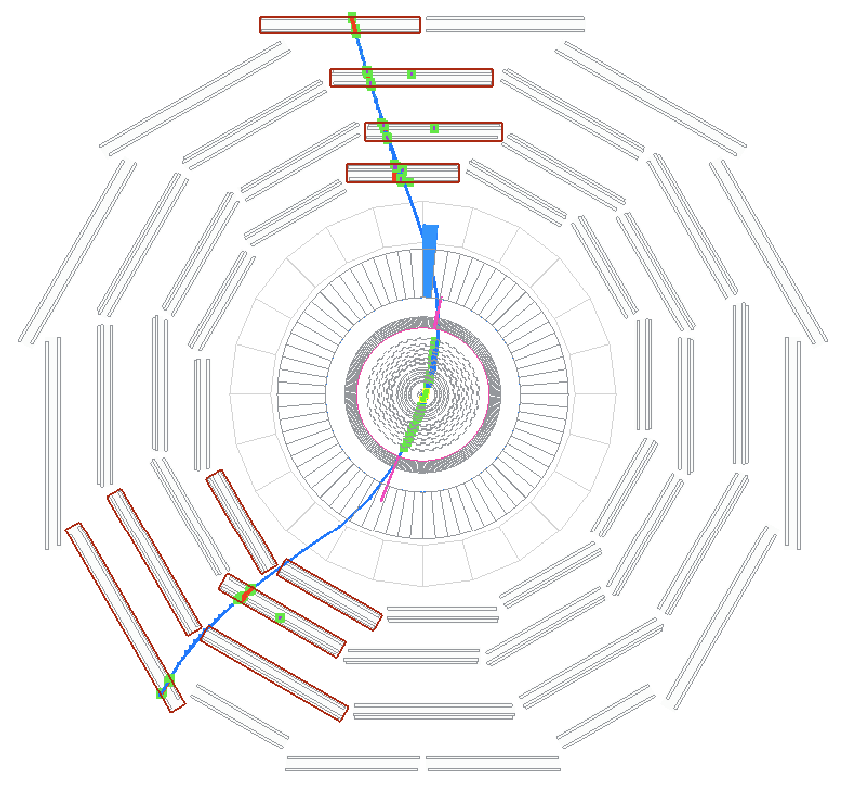
\includegraphics[width=0.5\linewidth]{event_display.png}
%% \end{center}

%% \begin{itemize}
%% \item We've all seen event displays, so we know that tracking \mbox{basically works\hspace{-1 cm}}
%% \item Now we need to use the millions of cosmic rays to test and correct tracking with high precision
%% \end{itemize}
%% %% \hspace{-0.83 cm} \textcolor{darkblue}{\Large Outline2}
%% \end{frame}

%% \begin{frame}
%% \frametitle{Muon tracking}

%% \begin{columns}
%% \column{0.6\linewidth}
%% 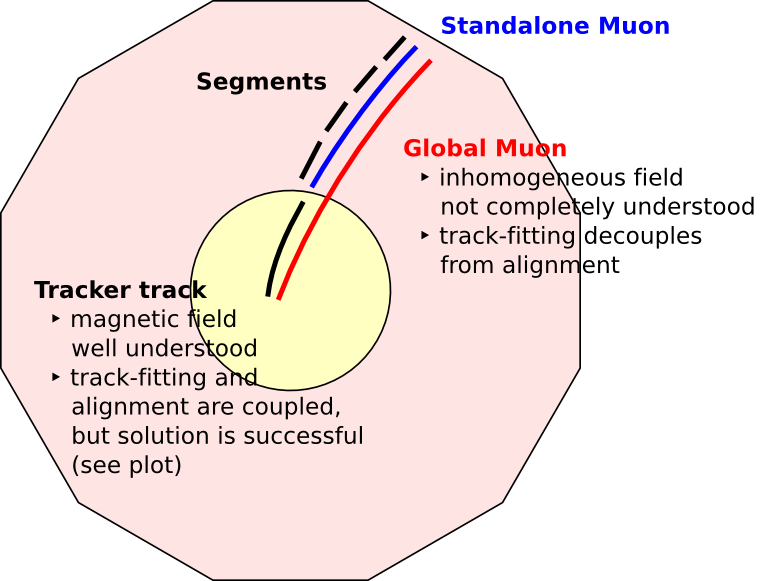
\includegraphics[width=\linewidth]{muon_tracks.png}

%% \column{0.5\linewidth}
%% \hfill \begin{minipage}{0.8\linewidth}
%% \tiny Tracker alignment group: J.\ Dr\"ger, R.\ Castello, G.\ Flucke, A.\ Gritsan, E.\ Migliore, M.\ Musich, A.\ Bonato, N.\ Tran, M.\ Weber et al.
%% \end{minipage}

%% 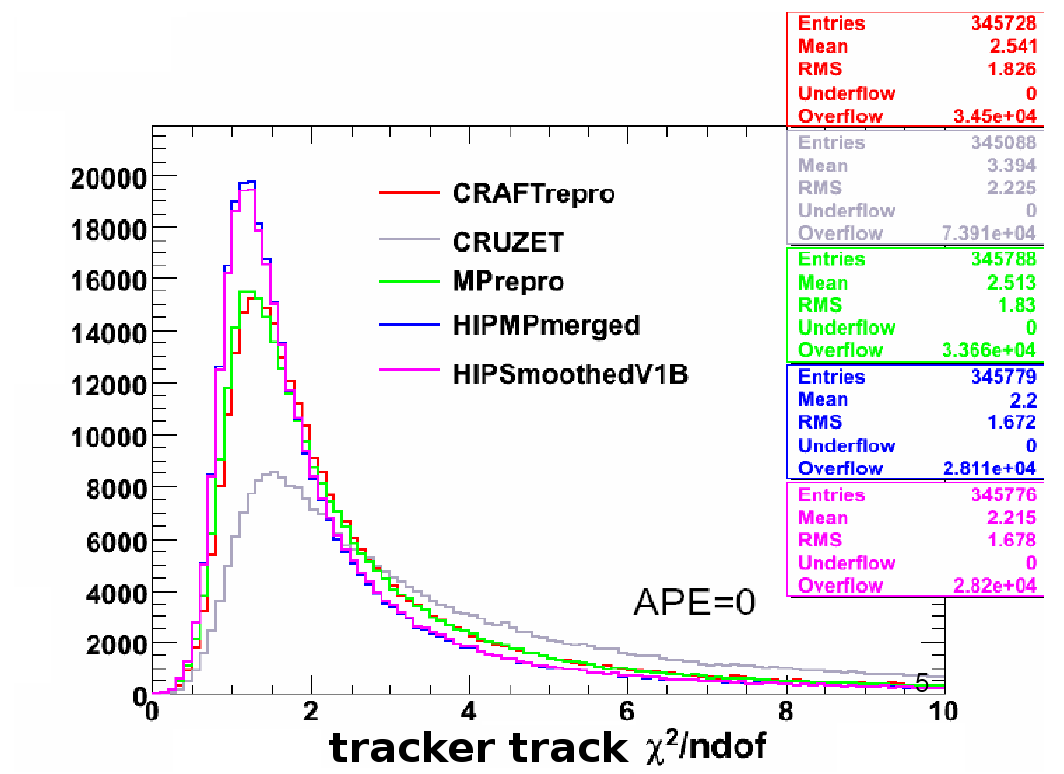
\includegraphics[width=\linewidth]{tracker_chi2.png}
%% \end{columns}

%% \vfill
%% \begin{itemize}
%% \item Precision generally proceeds from the tracker outward
%% \begin{itemize}\setlength{\itemsep}{0.2 cm}
%% \item successful tracker alignment provides a good platform from which
%%   to resolve unknown $\vec{B}(\vec{x})$ in the muon system
%% \end{itemize}
%% \item But also from local chamber segments outward
%% \item In both cases, the reference has a uniform magnetic field\ldots
%% \end{itemize}
%% \end{frame}

%% \begin{frame}
%% \frametitle{Indication of a problem}

%% \hfill {\tiny Nhan Tran, Alessio Bonato}

%% 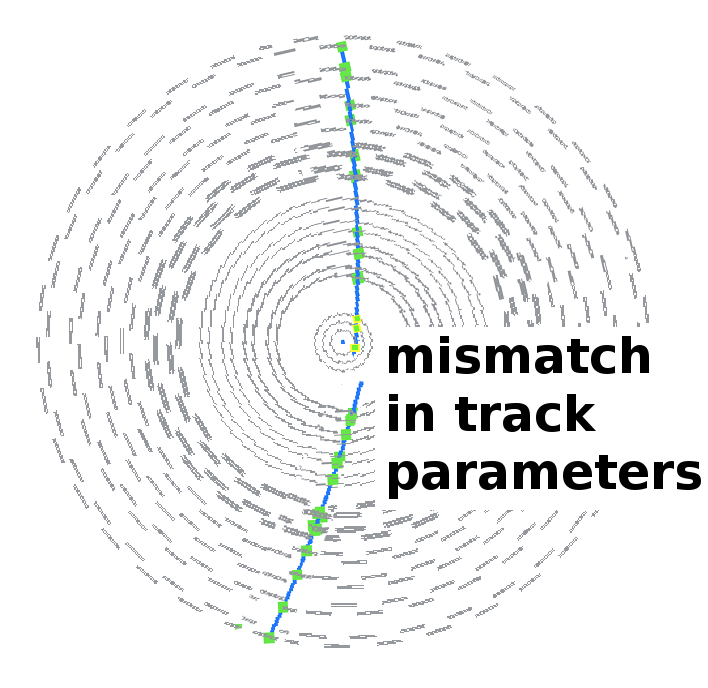
\includegraphics[height=2.6 cm]{matching.png} 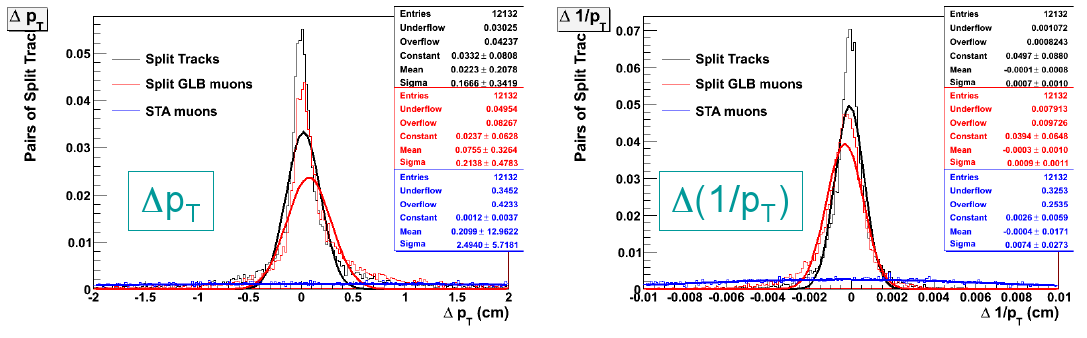
\includegraphics[height=2.6 cm]{mismatch2.png}

%% \begin{columns}
%% \column{0.3\linewidth}
%% \begin{itemize}
%% \item \mbox{Black: tracker track\hspace{-1 cm}}

%% \textcolor{red}{\mbox{Red: global muon\hspace{-1 cm}}}
%% \item Adding muon hits is not expected to help low-momentum tracks much, but it shouldn't hurt!
%% \end{itemize}

%% \column{0.75\linewidth}

%% 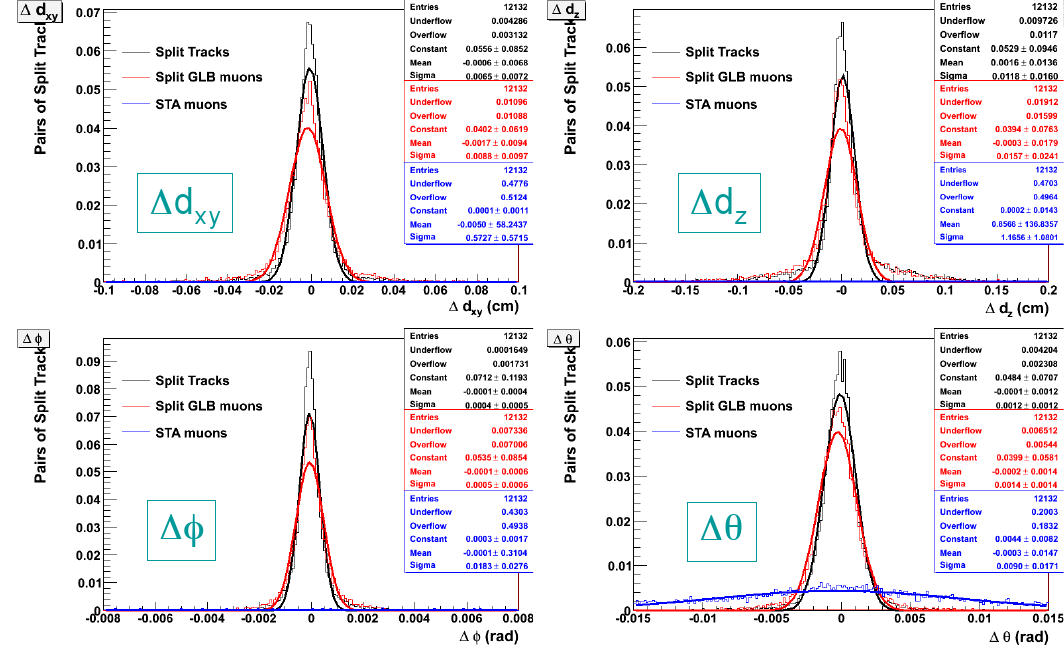
\includegraphics[width=\linewidth]{mismatch1.png}
%% \end{columns}
%% \end{frame}

%% \begin{frame}
%% \frametitle{Why is this important?}

%% \begin{itemize}
%% \item Why not use
%% \begin{itemize}
%% \item tracker for high-precision tracking
%% \item muon system for particle-id?
%% \end{itemize}

%% \item \textcolor{darkblue}{Answer:} because we care about high-momentum muons!

%% \mbox{ } \hfill 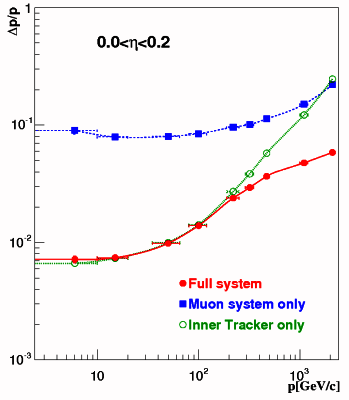
\includegraphics[width=0.35\linewidth]{Figure_001-005-a.png} 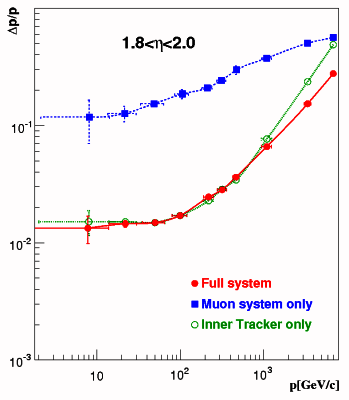
\includegraphics[width=0.35\linewidth]{Figure_001-005-b.png} \hfill {\tiny Physics TDR}

%% \item Solving muon tracking issues could make the difference between discovering $Z' \to \mu\mu$ in 2009/2010 and not having a significant peak

%% \item Heavy Stable Charged Particle searches also depend on good muon tracking for completely different reasons
%% \end{itemize}
%% \end{frame}

%% \begin{frame}
%% \frametitle{Muon tracking issues}

%% \begin{itemize}
%% \item \textcolor{darkblue}{\large Magnetic field map}
%% \begin{itemize}
%% \item exact shape of $\vec{B}(\vec{x})$ is difficult to model and depends on CMS's environment
%% \end{itemize}

%% \item \textcolor{darkblue}{\large Alignment}
%% \begin{itemize}
%% \item for the chambers' intrinsic resolution to be useful, their positions
%%   must be known with at least equal precision
%% \end{itemize}

%% \item \textcolor{darkblue}{\large Material budget}
%% \begin{itemize}
%% \item $dE/dx$ corrections are smaller, especially for high-momentum
%% \item treat as negligible for now
%% \end{itemize}

%% \item \textcolor{darkblue}{\large Calibration}
%% \begin{itemize}
%% \item can be solved independently of global tracking issues
%% \end{itemize}
%% \end{itemize}

%% \vfill
%% \hspace{-0.83 cm} \textcolor{darkblue}{\Large Outline for this talk}
%% \begin{enumerate}
%% \item What $\vec{B}$-field errors do to tracks
%% \item Aligning the muon system with an imperfectly-known field
%% \item Measuring the field corrections with an imperfectly-known alignment
%% \end{enumerate}
%% \end{frame}

%% \begin{frame}
%% \frametitle{Knowledge of magnetic field}

%% \textcolor{darkblue}{\large \ldots inside the solenoid}

%% \begin{center}
%% \begin{minipage}{0.9\linewidth}
%% \begin{itemize}
%% \item Magnetic field mapper, NMR probes's 2006 and 2008 data, and simulation all agree at the 0.1\% level
%% \end{itemize}
%% \end{minipage}
%% \end{center}

%% \vfill
%% \textcolor{darkblue}{\large \ldots in the far reaches of the muon system}
%% \begin{center}
%% \begin{minipage}{0.9\linewidth}
%% \begin{itemize}
%% \item Flux-loop measurements disagree with simulation as much as 20\% (2006 and 2008)
%% \item Forces on CASTOR were larger than expected
%% \item Evidence of $B_z$ errors in CRAFT tracks
%% \item Evidence of $B_r$ errors in CRAFT DT calibration
%% \end{itemize}
%% \end{minipage}
%% \end{center}
%% \end{frame}

%% \begin{frame}
%% \frametitle{Effect of $B_z$ errors on residuals}

%% \vfill
%% 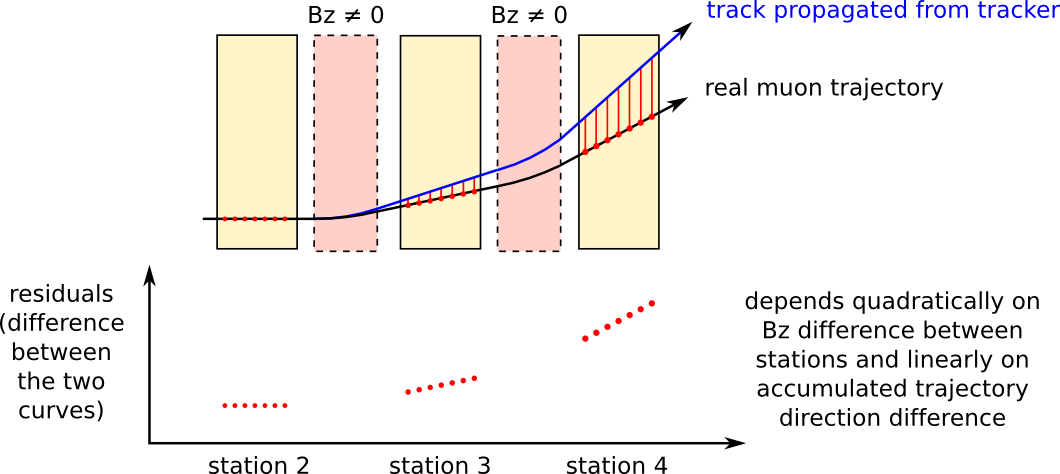
\includegraphics[width=\linewidth]{paths.png}

%% \vfill
%% \begin{itemize}
%% \item Gap between propagted track and real muon grows quadratically in yoke when $B_z$ is wrong
%% \item Gap grows linearly elsewhere, dependent on history

%% {\scriptsize (This is like a Physics I displacement problem with regions of acceleration)}
%% \end{itemize}
%% \end{frame}

%% \begin{frame}
%% \frametitle{Effect of $B_z$ errors on segments}

%% \vfill
%% 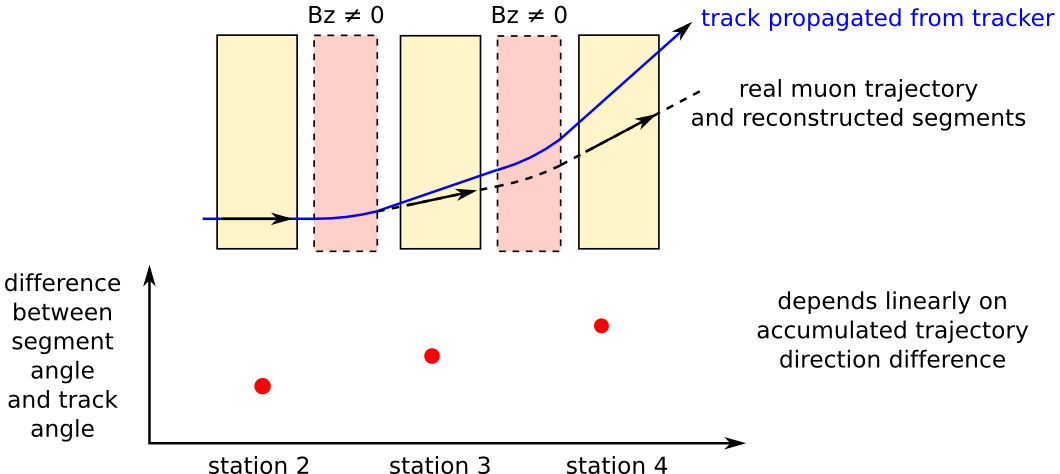
\includegraphics[width=\linewidth]{paths2.png}

%% \vfill
%% \begin{itemize}
%% \item Trajectory angle grows linearly in yoke when $B_z$ is wrong

%% {\scriptsize (This is like a Physics I velocity problem with regions of acceleration)}

%% \item Difference in segment angles on the same track provides a direct measurement of $B_z$ error
%% \item Residuals method can provide a cross-check
%% \end{itemize}
%% \end{frame}

%% \begin{frame}
%% \frametitle{What do we observe?}

%% \begin{columns}
%% \column{0.5\linewidth}
%% \begin{center}
%% \textcolor{darkblue}{\large Residuals}
%% \end{center}

%% 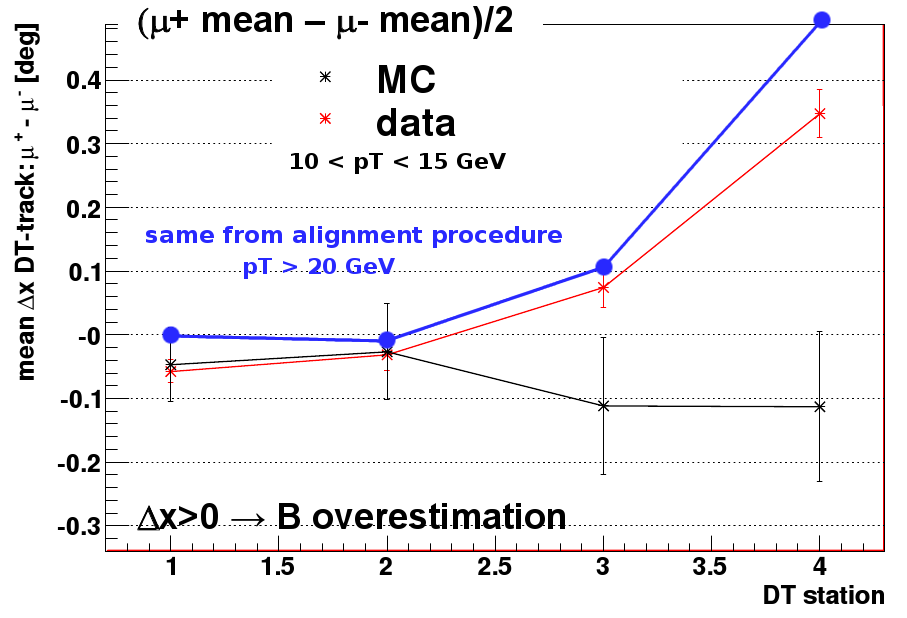
\includegraphics[height=3.5 cm]{sara_position_method_withalignment.png}

%% \hfill {\tiny Sara Bolognesi, blue points: Jim Pivarski}

%% \column{0.5\linewidth}
%% \begin{center}
%% \textcolor{darkblue}{\large Segment angles}
%% \end{center}

%% 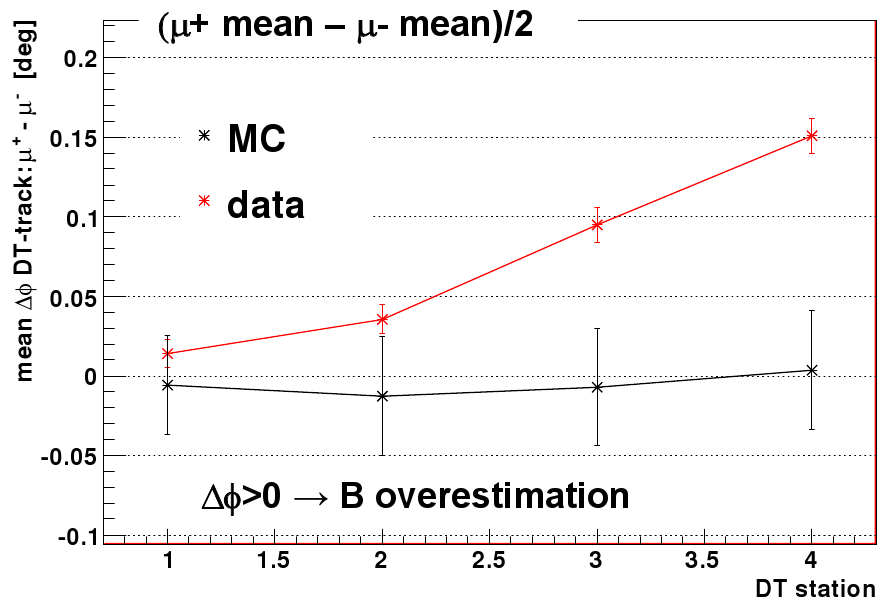
\includegraphics[height=3.5 cm]{sara_angle_method.png}

%% \hfill {\tiny Sara Bolognesi}
%% \end{columns}

%% \vfill
%% \begin{itemize}
%% \item Plots show integrated effect from tracker to each station
%% \item Also shown to be $\phi$ and $z$ symmetric within each station
%% \item Real magnetic field is {\it smaller} than what is used in the simulation
%% \end{itemize}
%% \end{frame}

%% \begin{frame}
%% \frametitle{$B_z$ error and alignment}

%% \begin{columns}
%% \column{0.6\linewidth}

%% \begin{itemize}\setlength{\itemsep}{0.35 cm}
%% \item Residuals from $B_z$ error are \mbox{as large as 5~mm\hspace{-1 cm}}
%% \item Residuals from chamber misalignment \mbox{were 5--10~mm\hspace{-3 cm}}
%% \item How can we disentangle them?
%% \begin{itemize}\setlength{\itemsep}{0.2 cm}
%% \item magnetic field effect depends on momentum and is antisymmetric with charge

%% $\displaystyle \mbox{residual} = \textcolor{darkblue}{(q/p_T)} \, \frac{\ell^2}{\mbox{600 cm}} \, \Delta B$

%% \item misalignment effect is independent of momentum
%% \end{itemize}
%% \item Residuals versus curvature ($q/p_T$):
%% \begin{itemize}
%% \item $B_z$ error introduces \mbox{slope\hspace{-1 cm}}
%% \item misalignment is the value at infinite momentum ($q/p_T \to 0$)
%% \end{itemize}
%% \end{itemize}

%% \column{0.4\linewidth}
%% \hfill 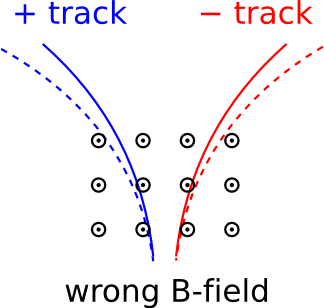
\includegraphics[width=0.6\linewidth]{antisymmetric_bfield.png}

%% \vspace{0.5 cm}
%% 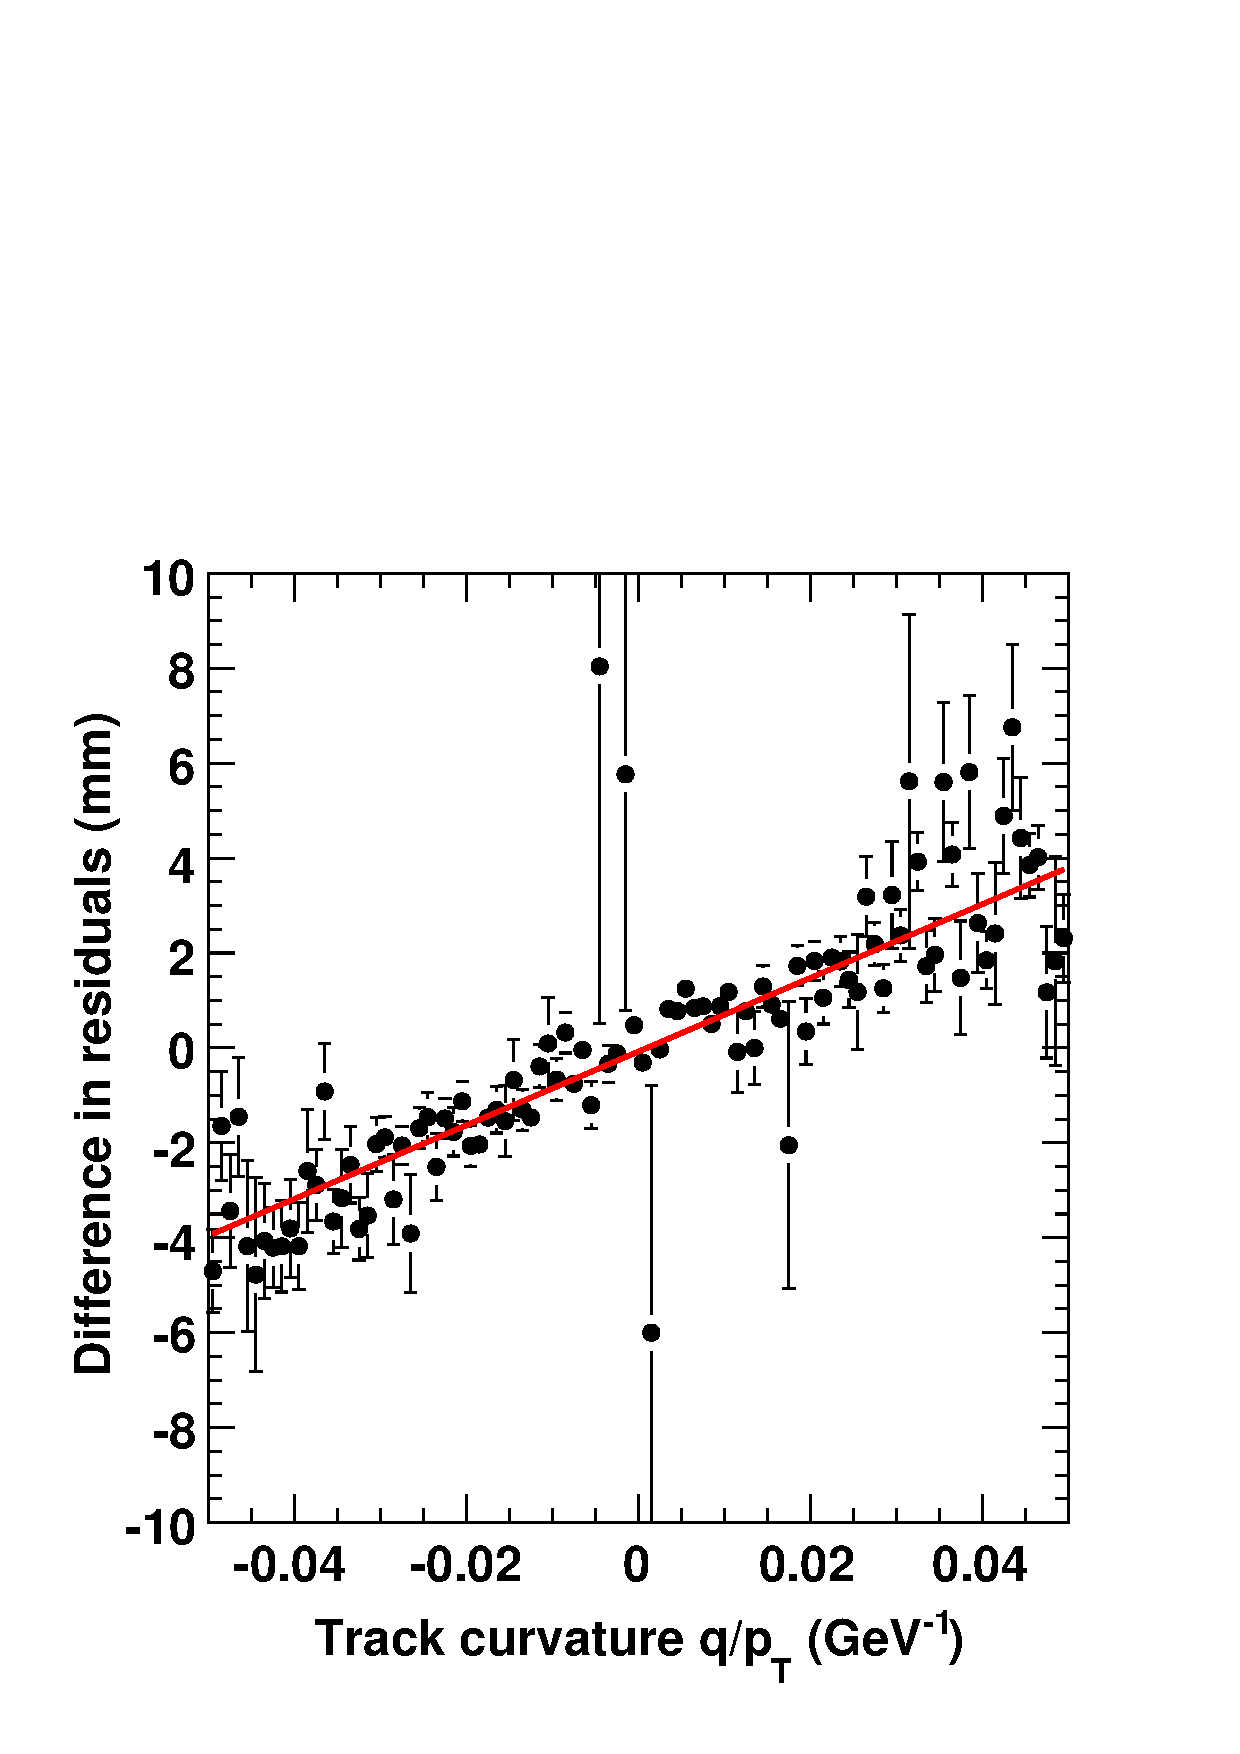
\includegraphics[width=\linewidth]{demo_qoverpt.pdf}
%% \end{columns}

%% \end{frame}

%% \begin{frame}
%% \frametitle{Measuring alignment}
%% \framesubtitle{(magnetic field is a controlled systematic error)}

%% \begin{columns}
%% \column{0.3\linewidth}
%% 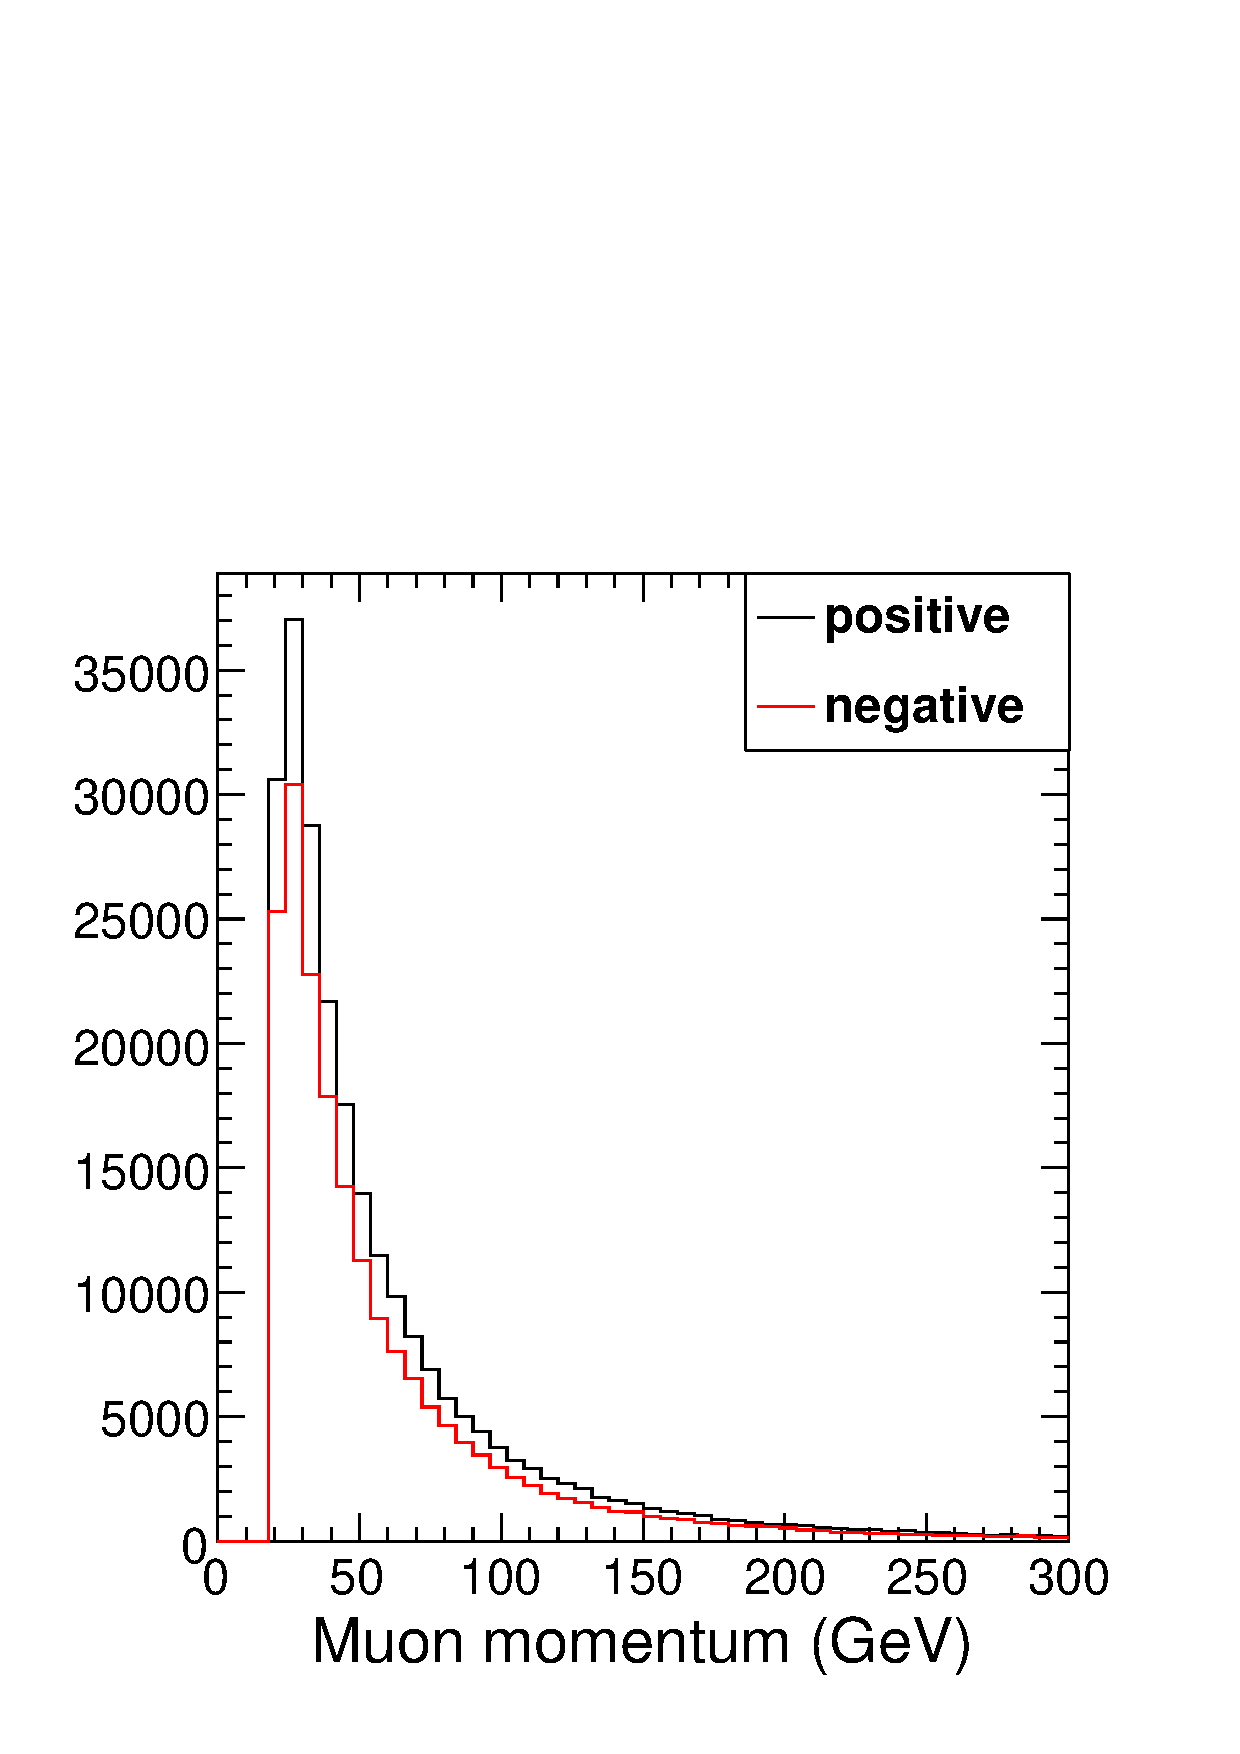
\includegraphics[width=\linewidth]{demo_momentum.pdf}

%% 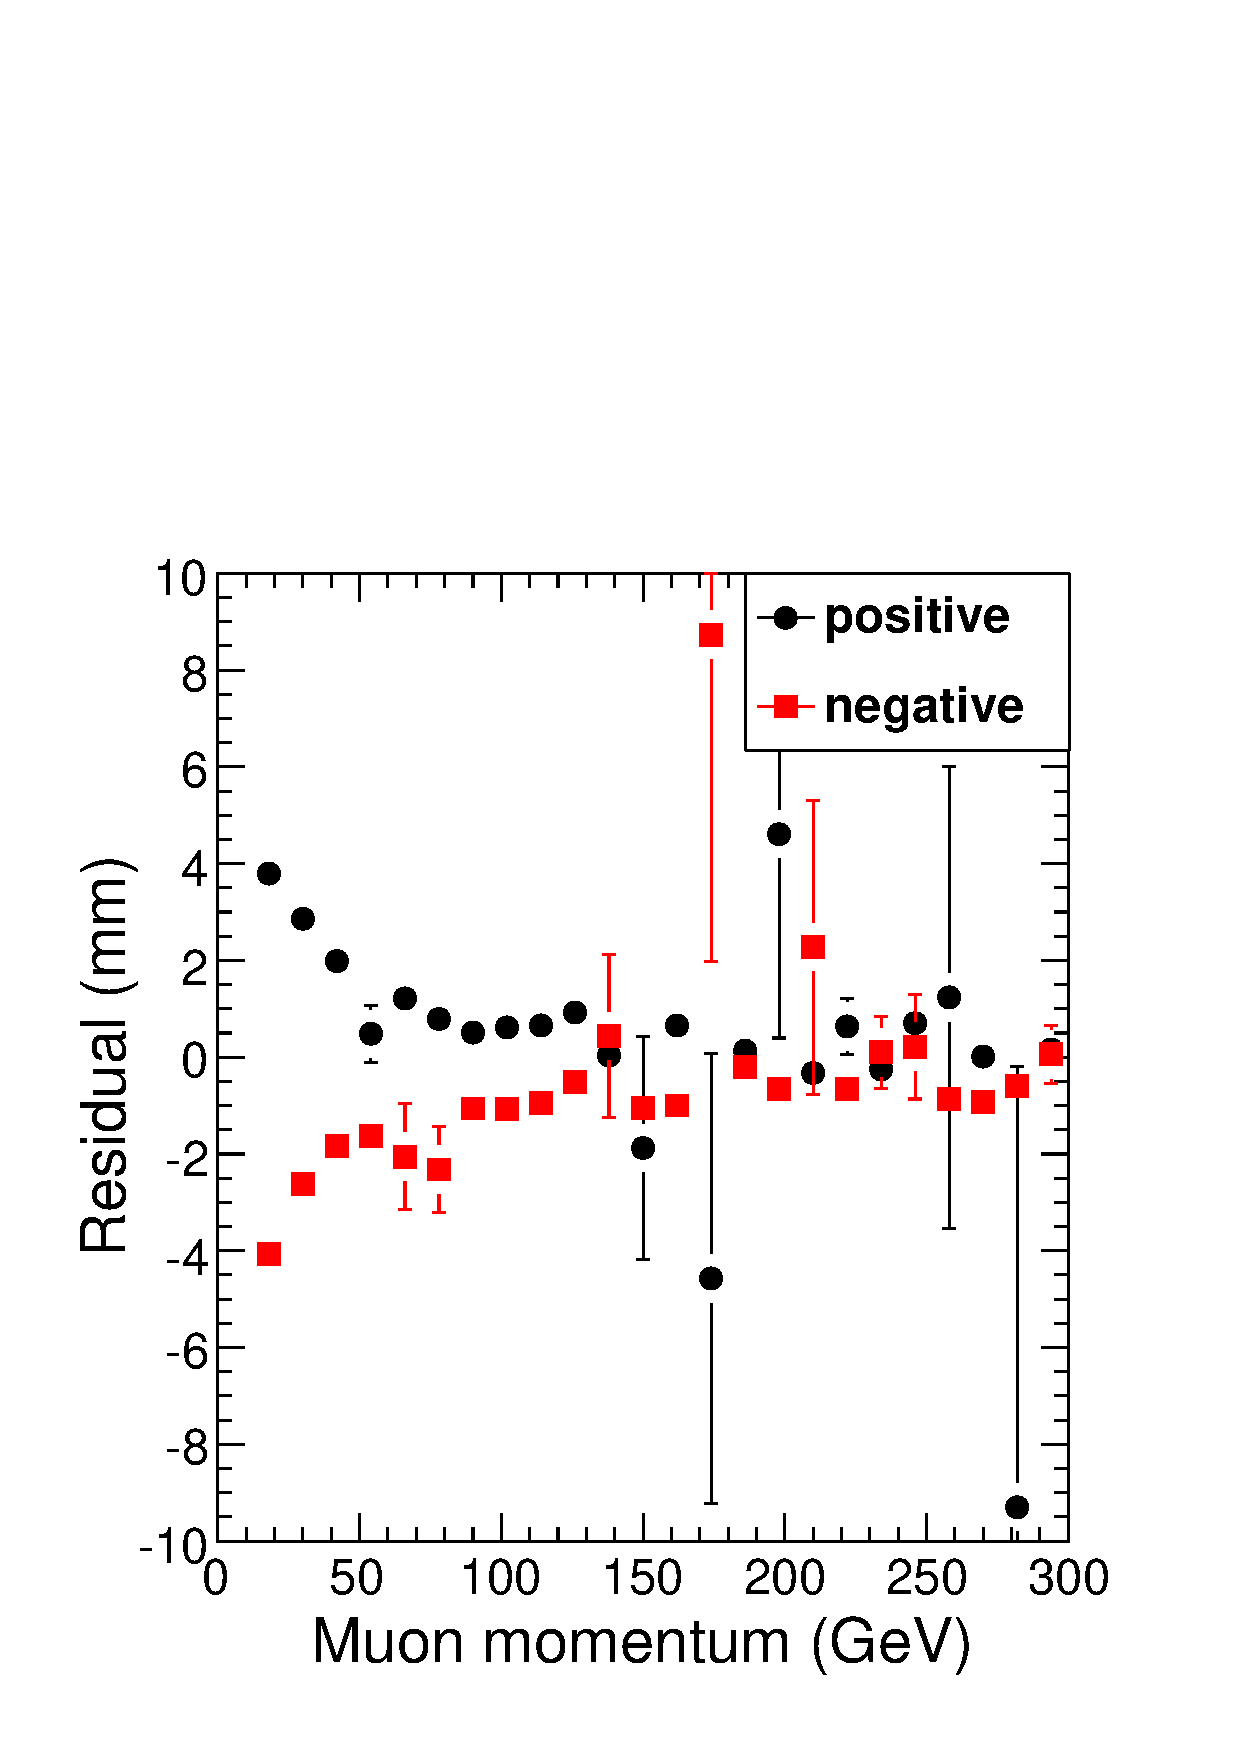
\includegraphics[width=\linewidth]{demo_residual.pdf} 
%% \column{0.7\linewidth}
%% \mbox{\hspace{-1.3 cm}\begin{minipage}{1.2\linewidth}
%% \begin{description}
%% \item[Fact:] Momentum spectra for positively-charged and negatively-charged cosmic rays are equal, though the number of each differ \\ (used in Cosmic Charge Ratio Analysis)
%% \item[Fact:] Effect of $\vec{B}$ on residuals flips sign with charge
%% \end{description}
%% \end{minipage}}

%% \vspace{0.3 cm}
%% \begin{itemize}\setlength{\itemsep}{0.1 cm}
%% \item Find peak of residuals in two bins: \\ $R_+$ (positively-charged) and $R_-$ \mbox{(negative)\hspace{-1 cm}}
%% \item Misalignment residual $\equiv$ $\displaystyle \frac{R_+ + R_-}{2}$
%% \begin{itemize}
%% \item effectively scales up negatively-charged population to cancel effect of positives
%% \end{itemize}
%% \item Syst.\ $=$ \mbox{$\displaystyle \left(\frac{R_+ - R_-}{2}\right) \, (\mbox{charge confusion}) \times \frac{0.3}{2.3}$\hspace{-2 cm}}
%% \begin{itemize}
%% \item Always plot $(R_+ - R_-)/2$ to trace systematic error (times a large factor)
%% \end{itemize}
%% \end{itemize}

%% \end{columns}
%% \end{frame}

%% \begin{frame}
%% \frametitle{Demonstration in station 4}

%% \begin{itemize}
%% \item Station 4 has the largest $\vec{B}$-field errors: plot residuals across barrel
%% \item The \textcolor{darkred}{misalignment measure} breaks cleanly at the \mbox{chamber boundaries\hspace{-1 cm}}
%% \item The \textcolor{lightblue}{tracer of $\vec{B}$-field errors} is independent of chamber
%% \end{itemize}

%% 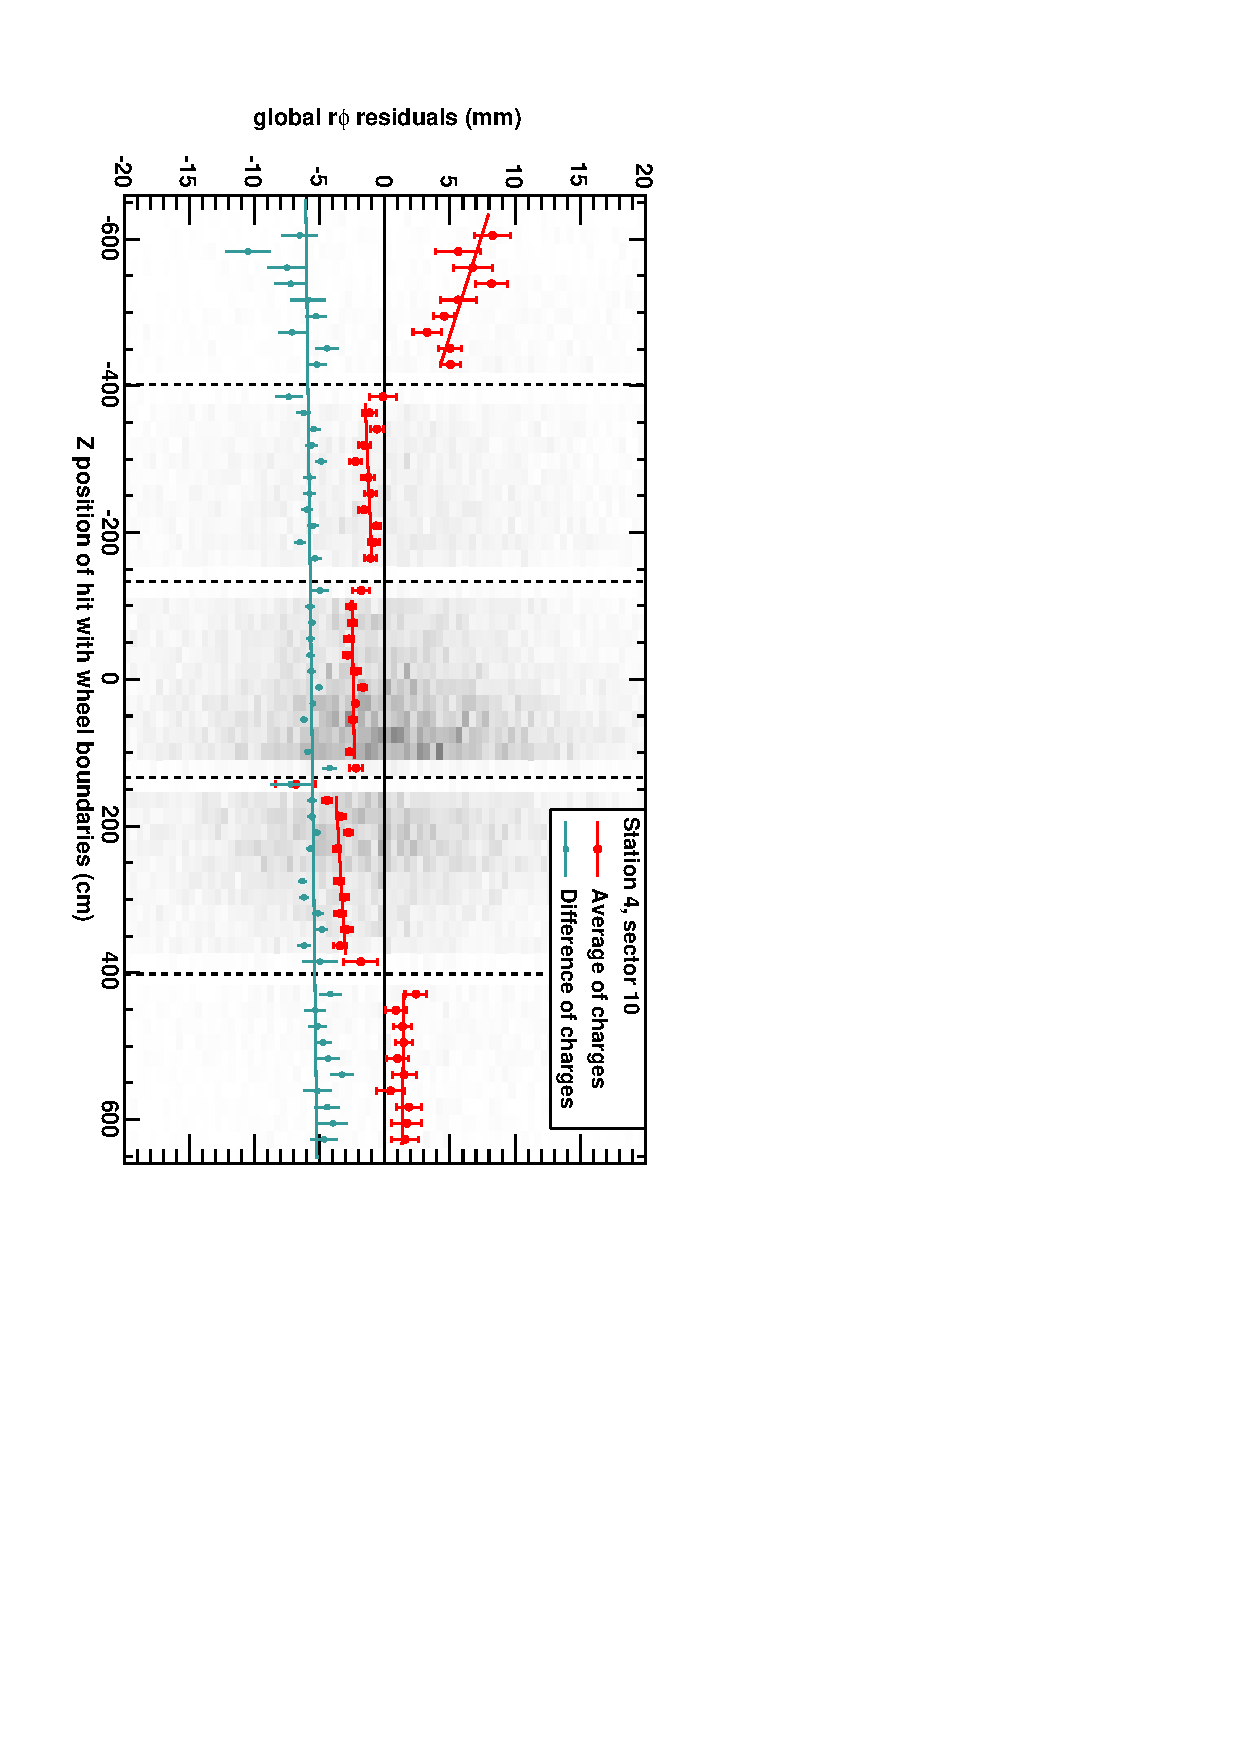
\includegraphics[height=\linewidth, angle=90]{demo_of_bfield.pdf}

%% \scriptsize grey background is the raw 2-D residuals distribution

%% linear fits are only a guide for the eye: not used in alignment!
%% \end{frame}

%% \begin{frame}
%% \frametitle{Alignment validation}

%% \vspace{0.3 cm}
%% Same story when viewed as a function of $\phi$ \mbox{(wheel 0 shown for four stations)\hspace{-1 cm}}

%% \mbox{ } \hfill \begin{minipage}{0.85\linewidth}
%% 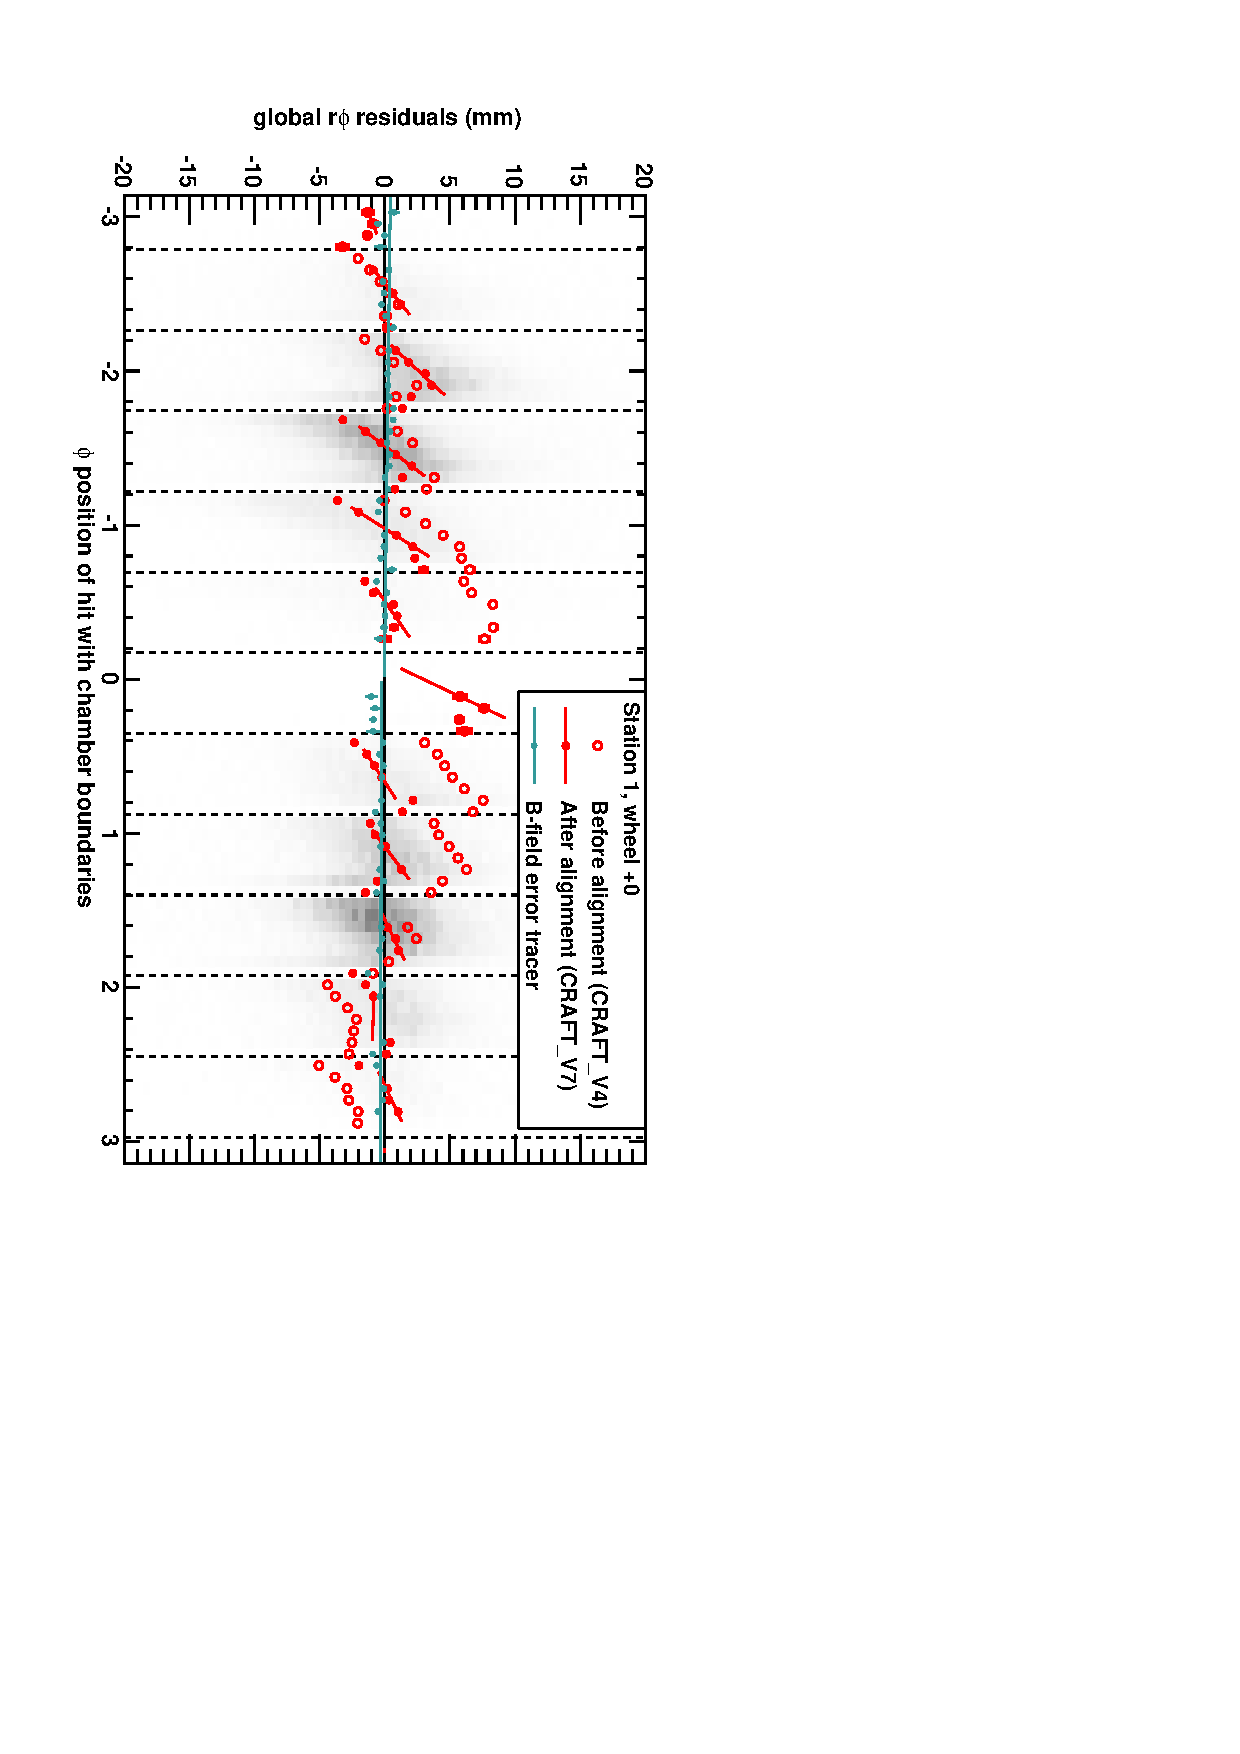
\includegraphics[height=0.5\linewidth, angle=90]{DTrphiVsPhi_st1_whC.pdf}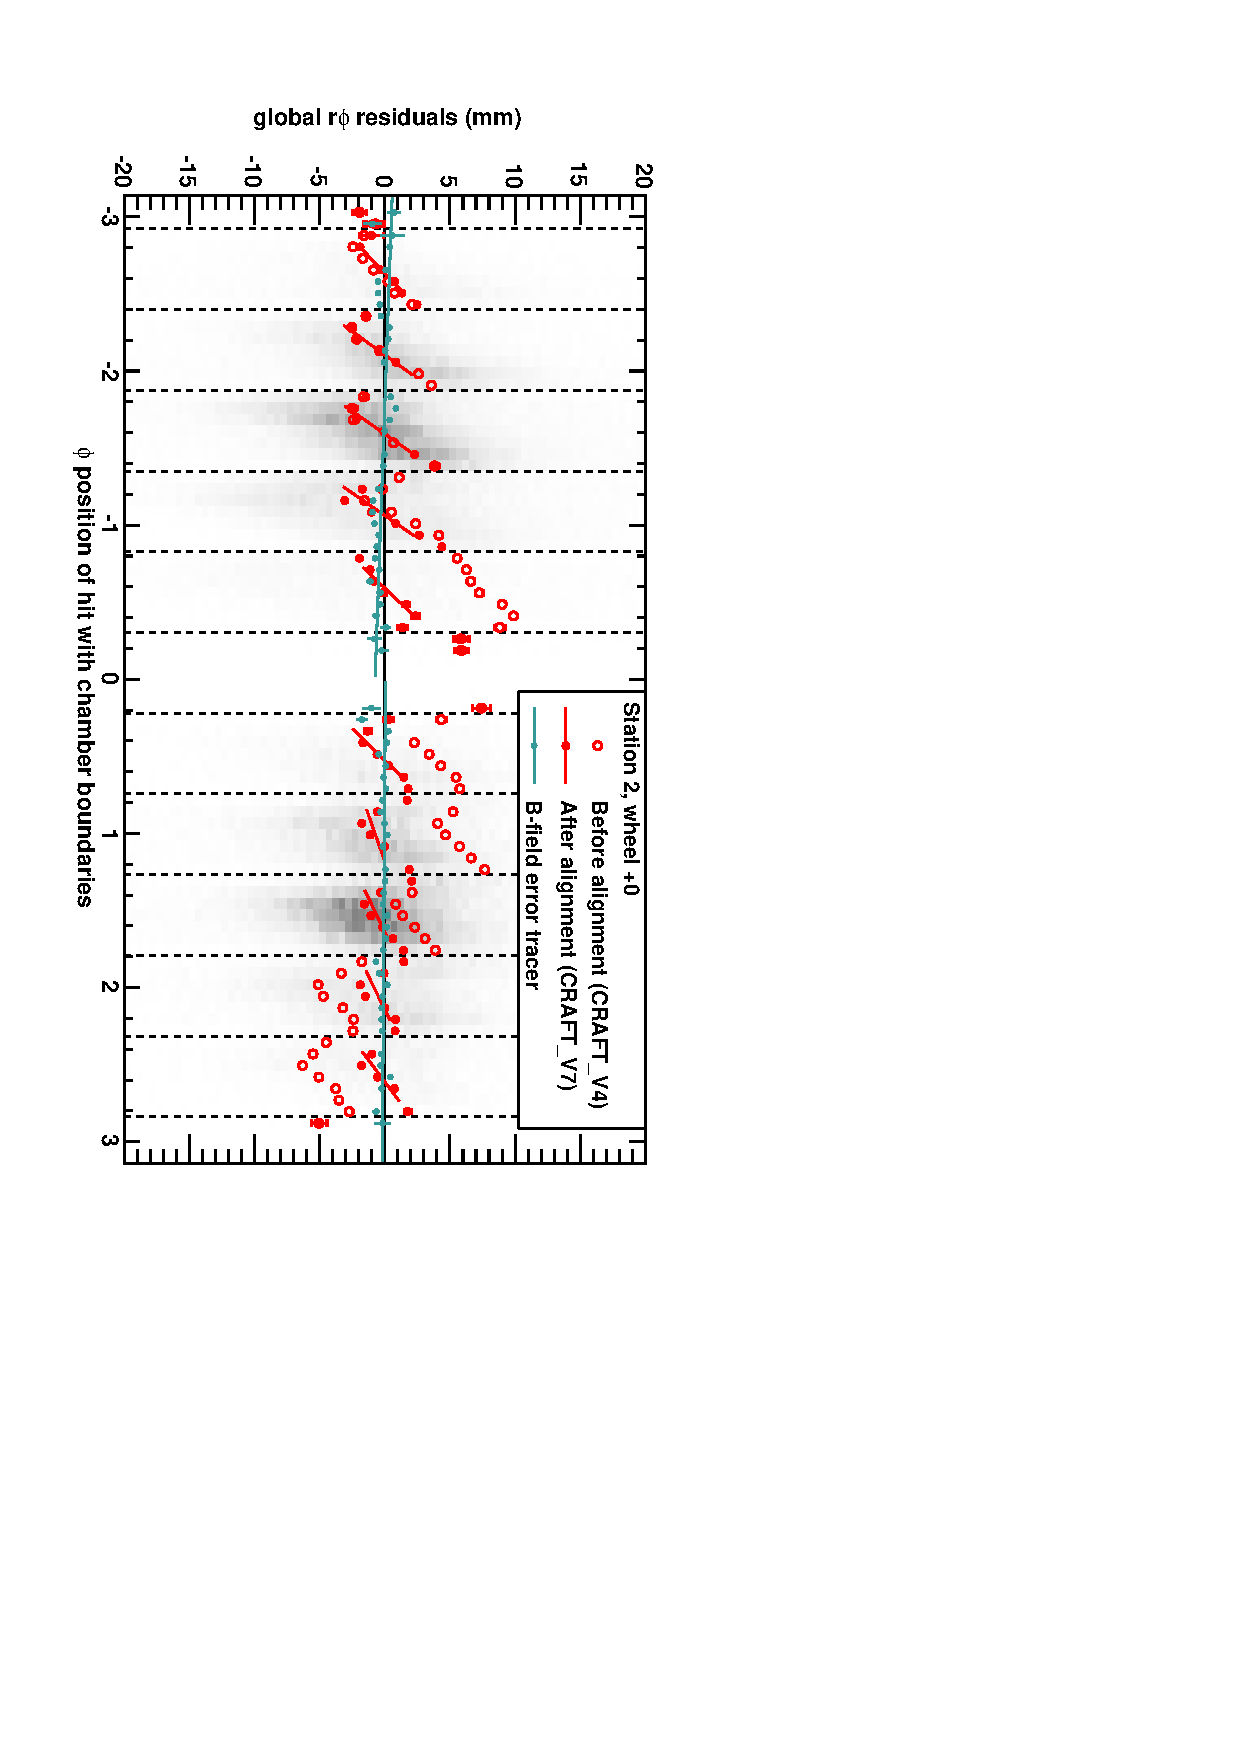
\includegraphics[height=0.5\linewidth, angle=90]{DTrphiVsPhi_st2_whC.pdf} \\
%% 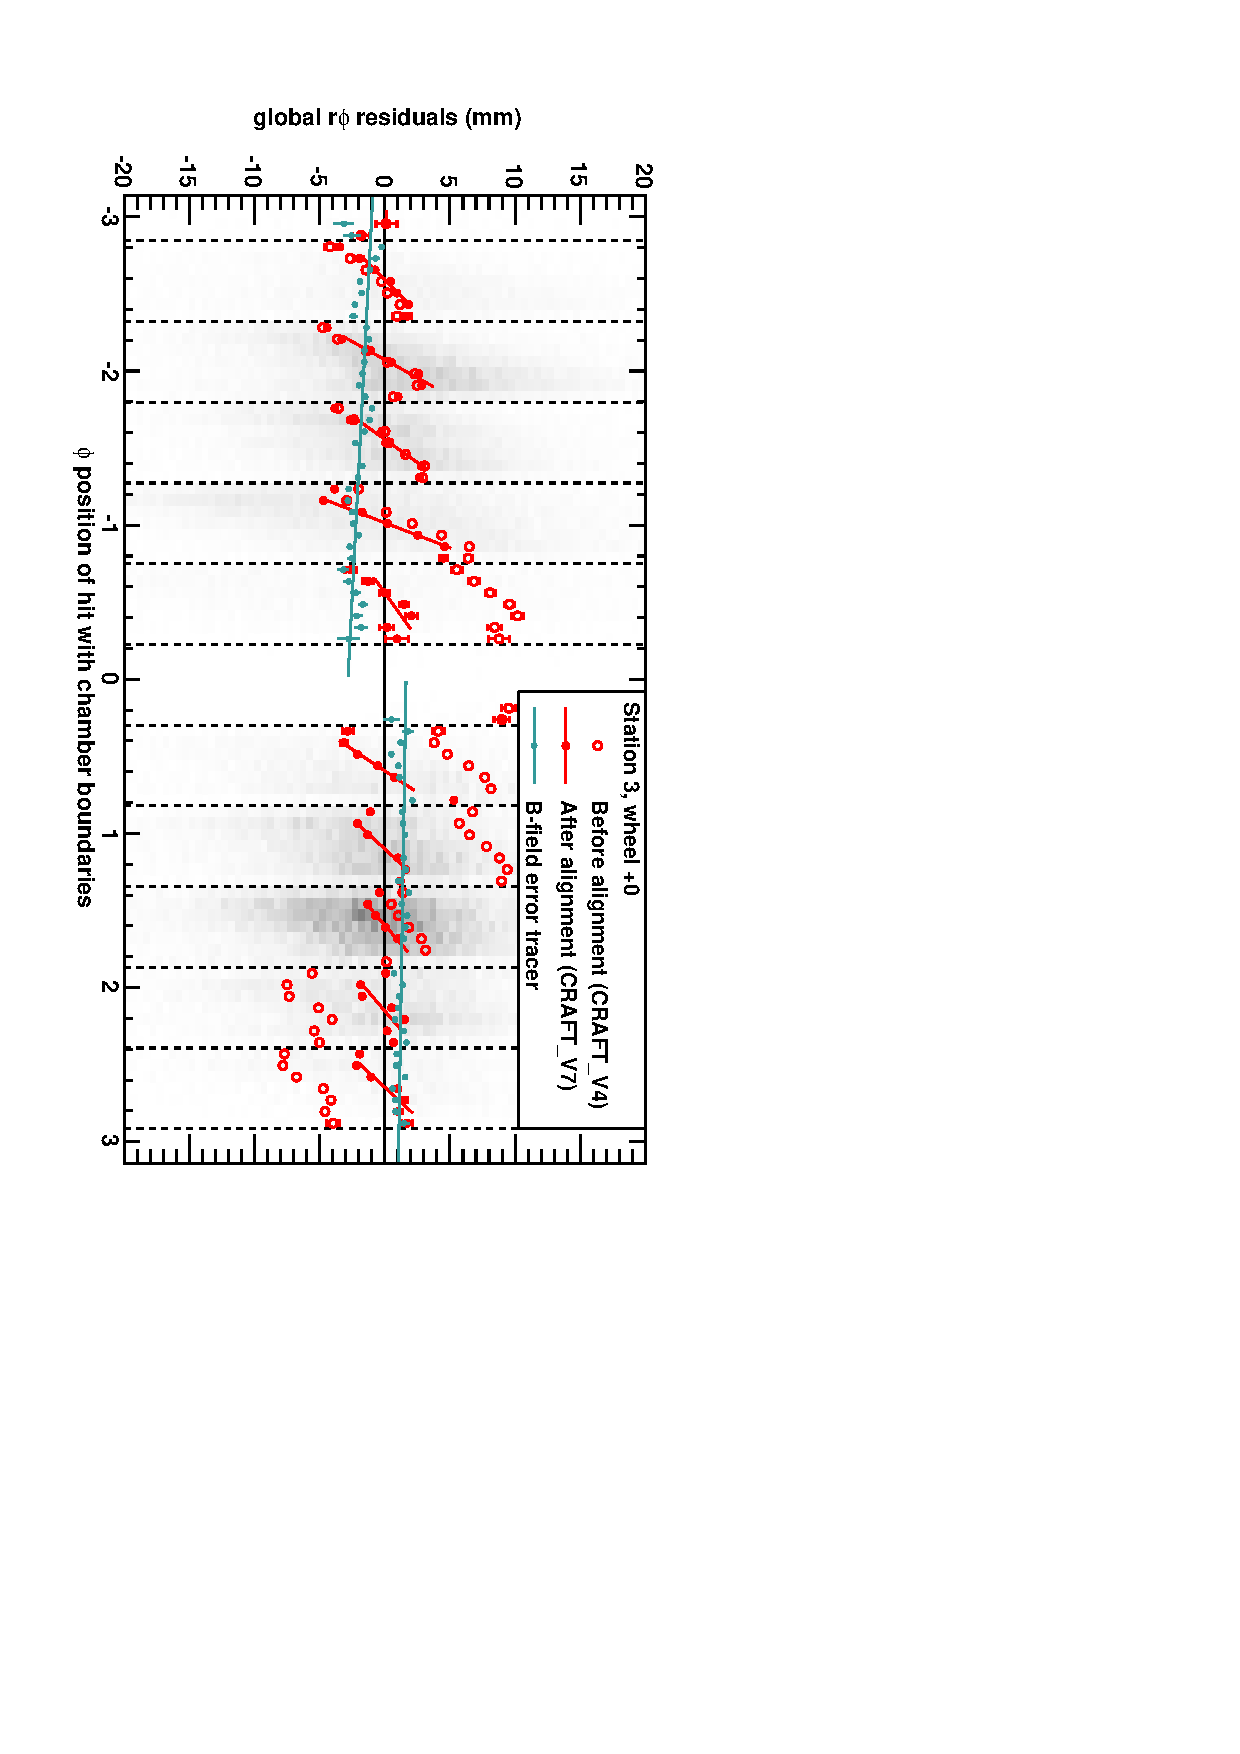
\includegraphics[height=0.5\linewidth, angle=90]{DTrphiVsPhi_st3_whC.pdf}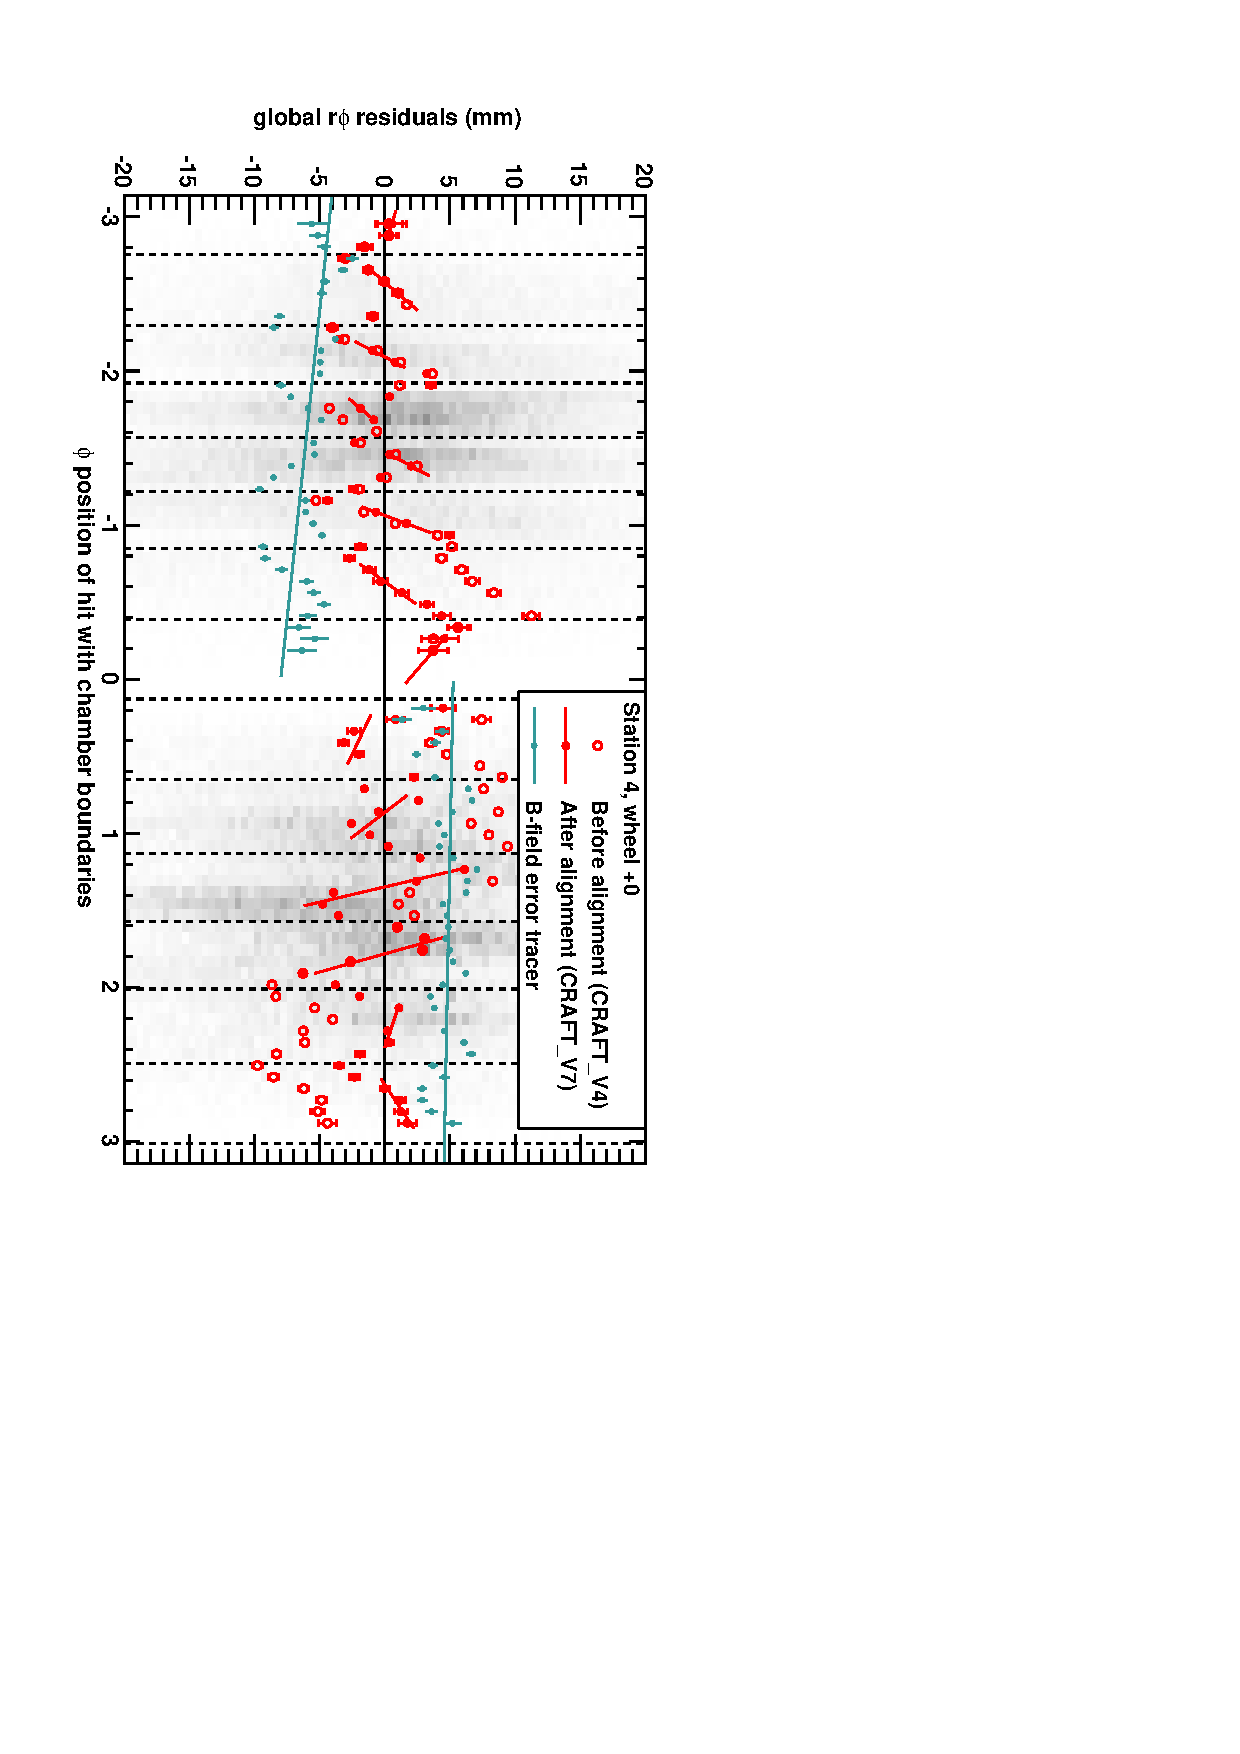
\includegraphics[height=0.5\linewidth, angle=90]{DTrphiVsPhi_st4_whC.pdf}
%% \end{minipage} \hfill \mbox{ }

%% \begin{itemize}
%% \item \textcolor{lightblue}{$(R_+ - R_-)/2$} non-negligible in stations 3 and 4 only
%% \item Flips sign in top of CMS ($\phi > 0$) because of direction of \mbox{muon velocity\hspace{-1 cm}}
%% \item Linear trend inside each chamber (sawtooth shape) is unexplained: early investigations indicate non-rigid distortion of DT chambers
%% \item See ``more information'' at \mbox{\textcolor{blue}{\tt \tiny \href{http://indico.cern.ch/conferenceDisplay.py?confId=51267}{http://indico.cern.ch/conferenceDisplay.py?confId=51267}}\hspace{-3 cm}}
%% \end{itemize}
%% \end{frame}

%% \begin{frame}
%% \frametitle{DT Alignment summary}
%% \begin{itemize}
%% \item Pattern of alignment corrections do not correspond to a rotation

%% 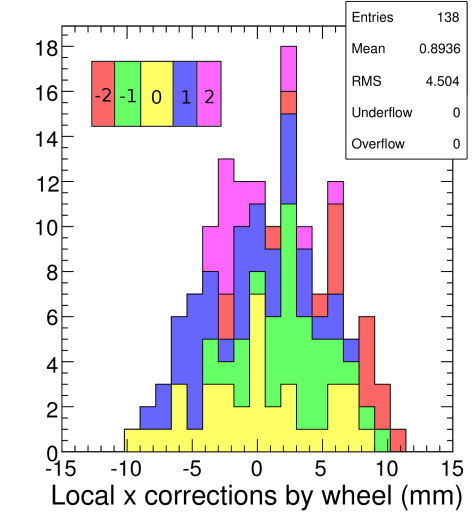
\includegraphics[width=0.25\linewidth]{report2_xbywheel.png} 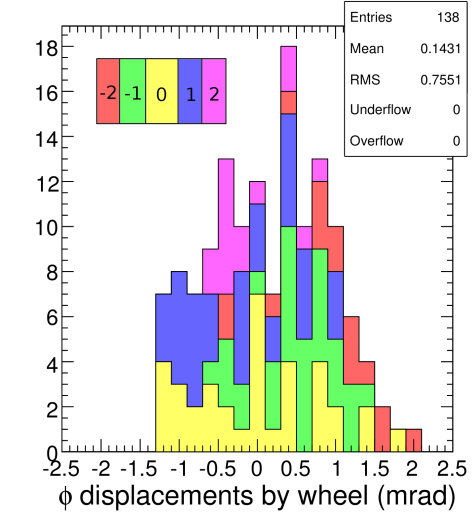
\includegraphics[width=0.25\linewidth]{report2_phibywheel.png} 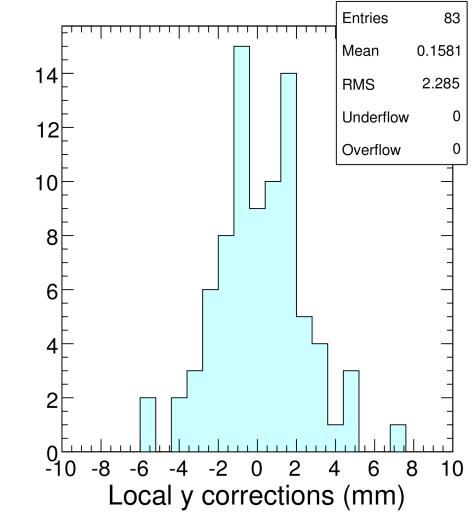
\includegraphics[width=0.25\linewidth]{report2_y.png} 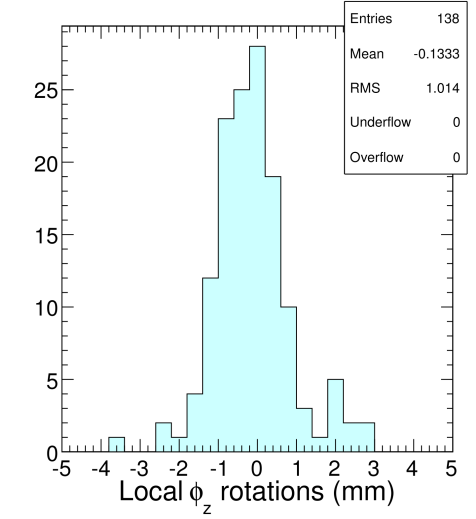
\includegraphics[width=0.25\linewidth]{report2_phiz.png}

%% \item Estimated residual misalignments: 1--2~mm \mbox{(a factor-of-five improvement)\hspace{-1 cm}}

%% \item Residuals visibly improve, despite unresolved ``sawtooth'' pattern

%% 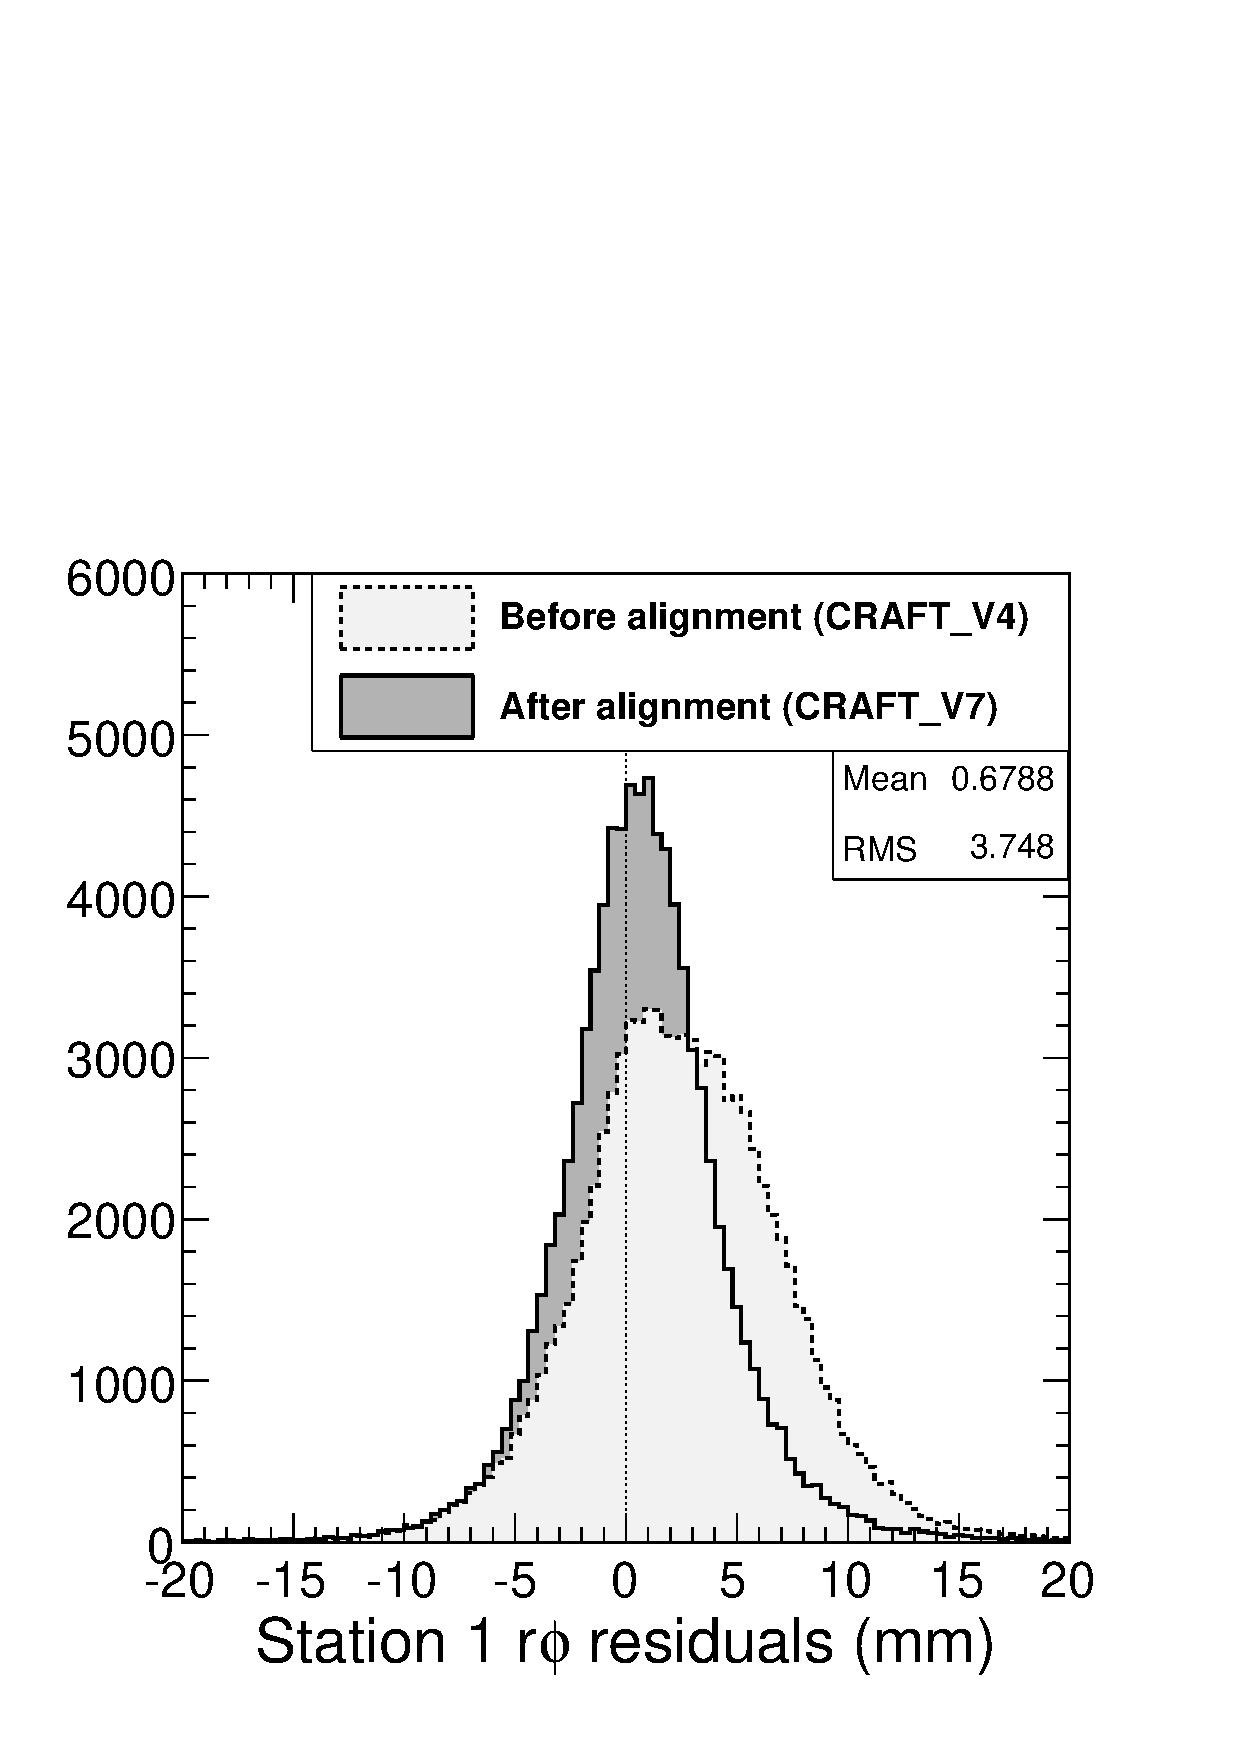
\includegraphics[width=0.25\linewidth]{residuals_improvement1.pdf} 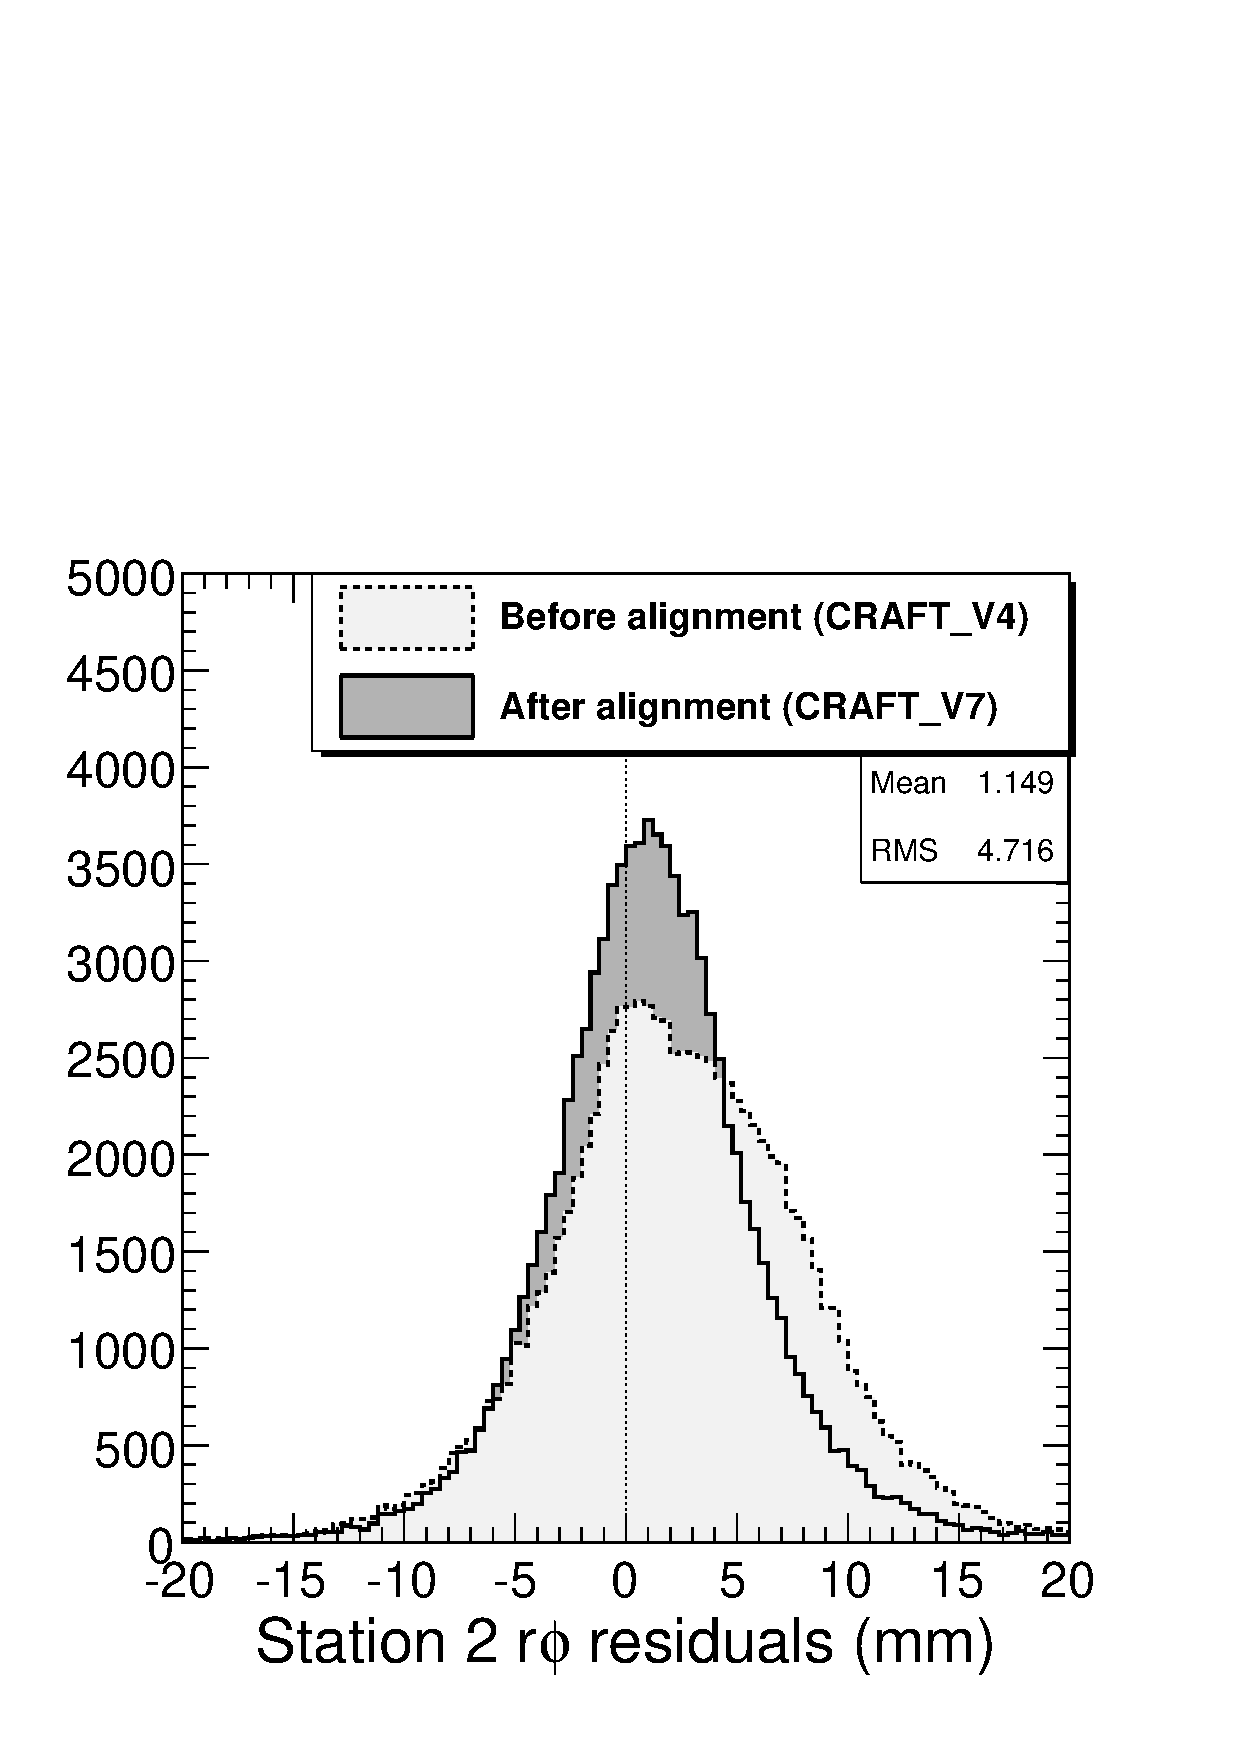
\includegraphics[width=0.25\linewidth]{residuals_improvement2.pdf} 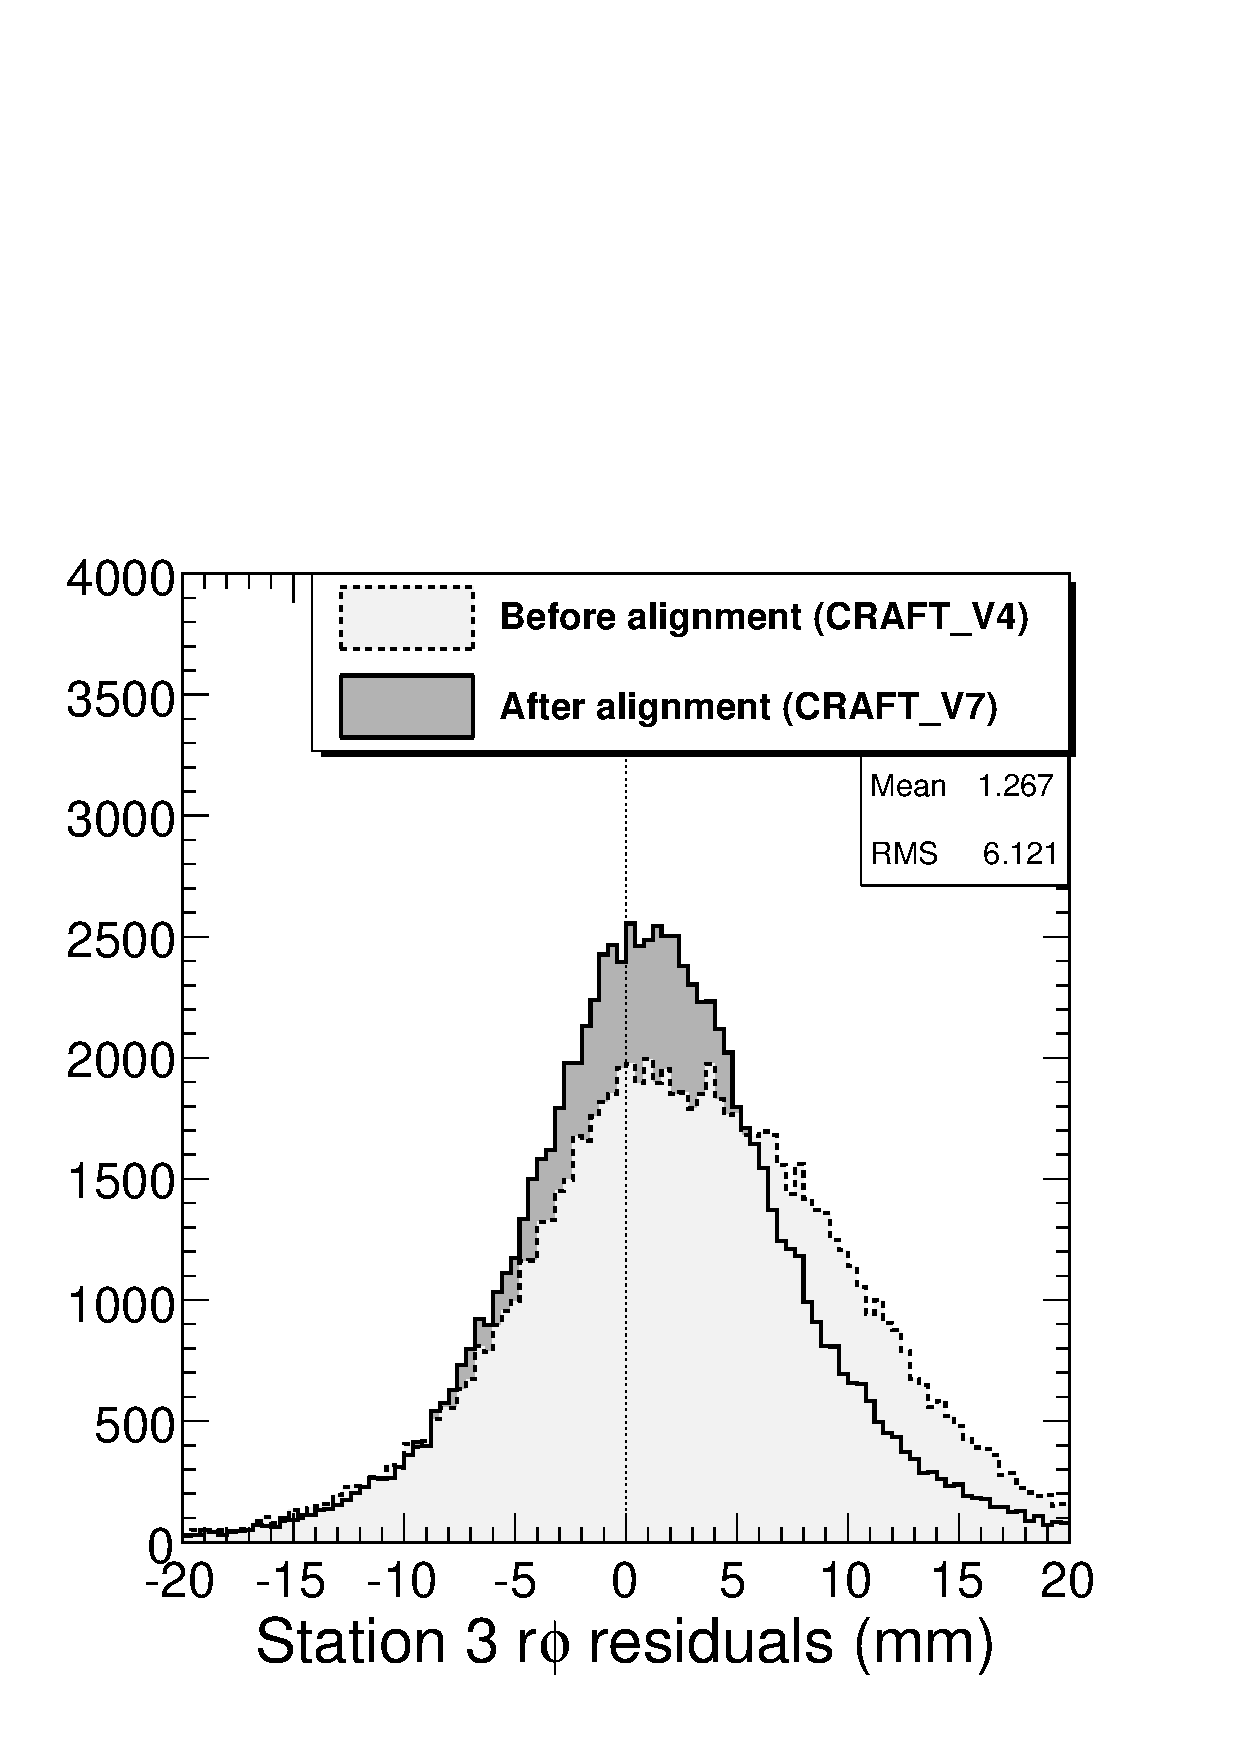
\includegraphics[width=0.25\linewidth]{residuals_improvement3.pdf} 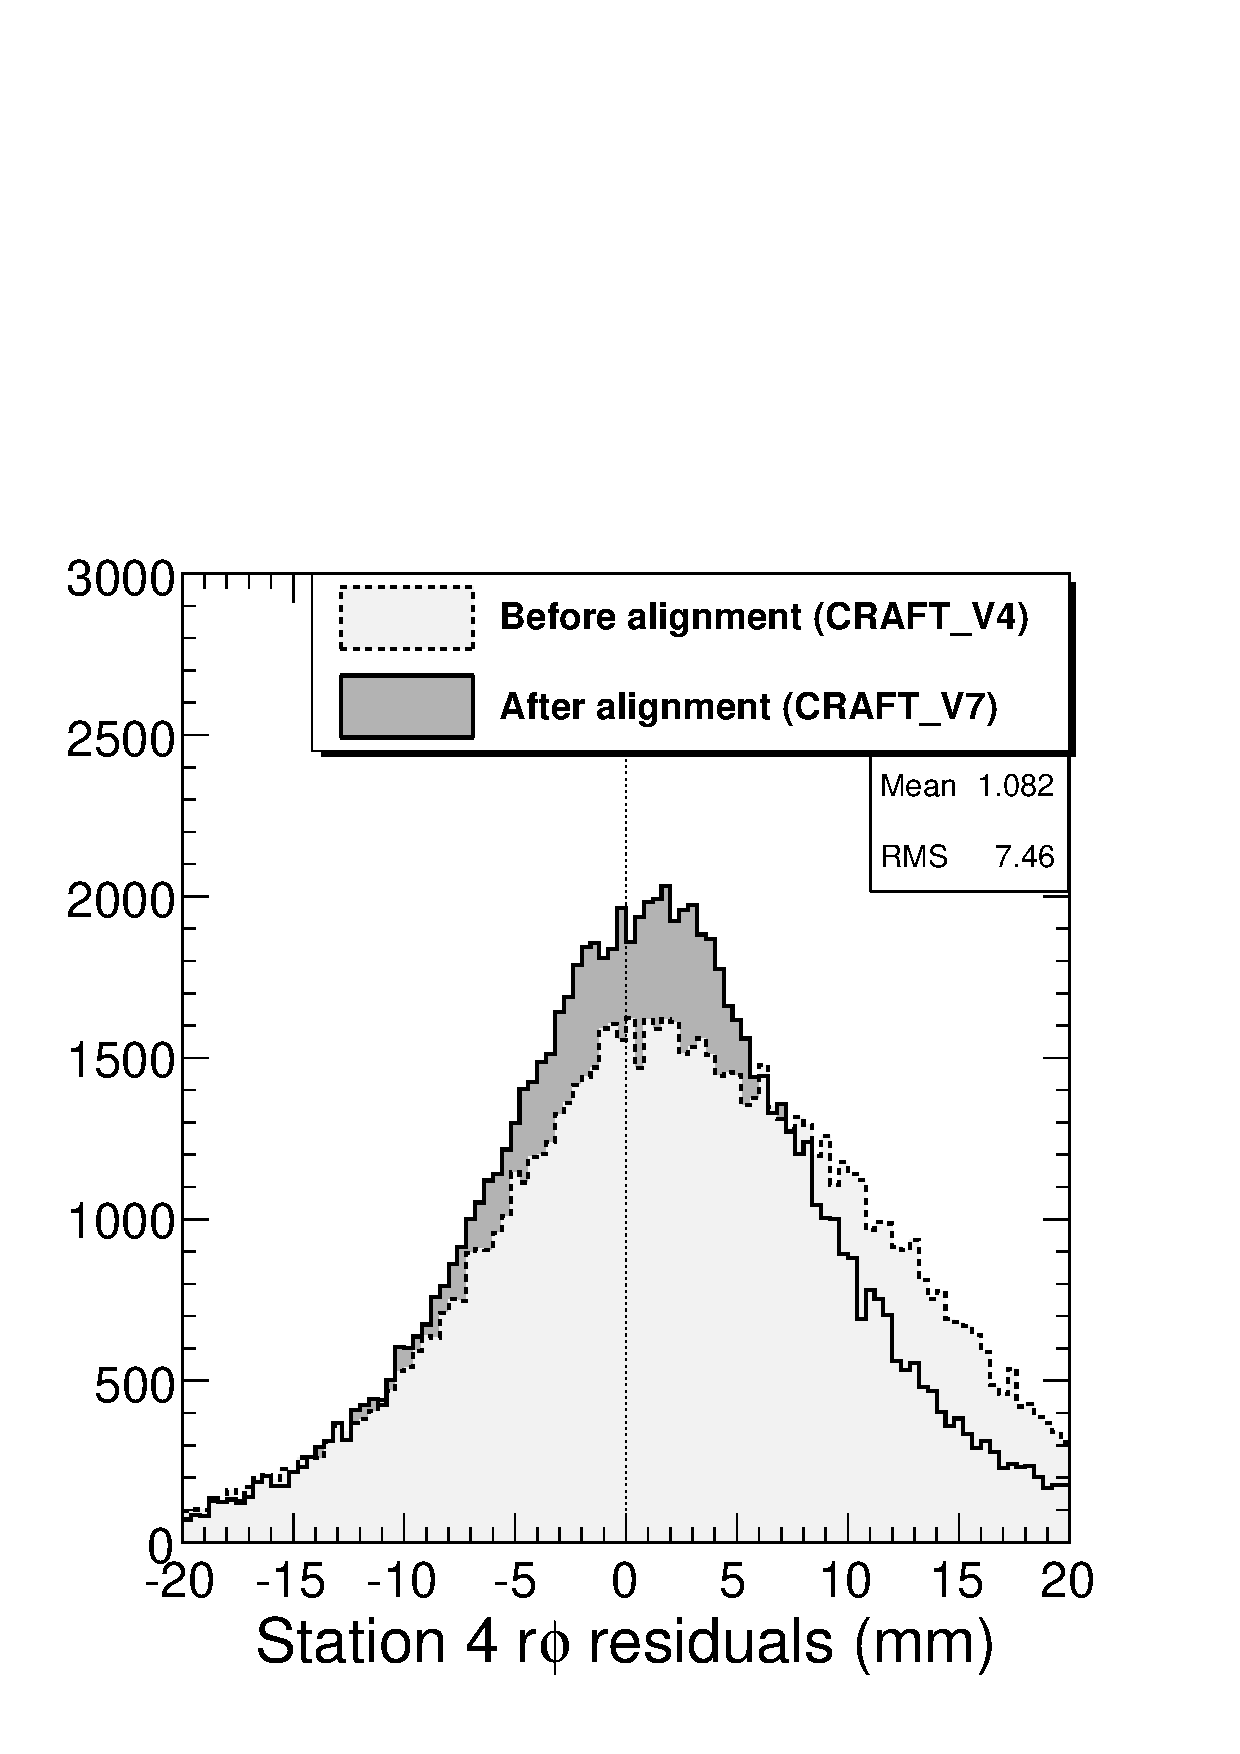
\includegraphics[width=0.25\linewidth]{residuals_improvement4.pdf}

%% \item CSCs are next, but will require a different technique due to vertical distribution of cosmic rays
%% \end{itemize}
%% \end{frame}

%% \begin{frame}
%% \frametitle{Measuring $B_z$ with segments}
%% \framesubtitle{(misalignment is a controlled systematic error)}

%% \vspace{0.5 cm}
%% \begin{columns}
%% \column{0.3\linewidth}
%% \begin{itemize}
%% \item Same principle: $B_z$ is isolated through the difference \mbox{between positive and negatively-\hspace{-3 cm}} \\ \mbox{charged bins, misalignment is\hspace{-3 cm}} \\ the average
%% \item \mbox{Instead of residuals, plot\hspace{-3 cm}} \\ \mbox{segment angle difference\hspace{-3 cm}} \\ \mbox{between two stations on the\hspace{-3 cm}} \\ same track
%% \item \mbox{Quantifies $B_z$ in the yoke\hspace{-3 cm}} \\ between them
%% \end{itemize}

%% \column{0.7\linewidth}
%% 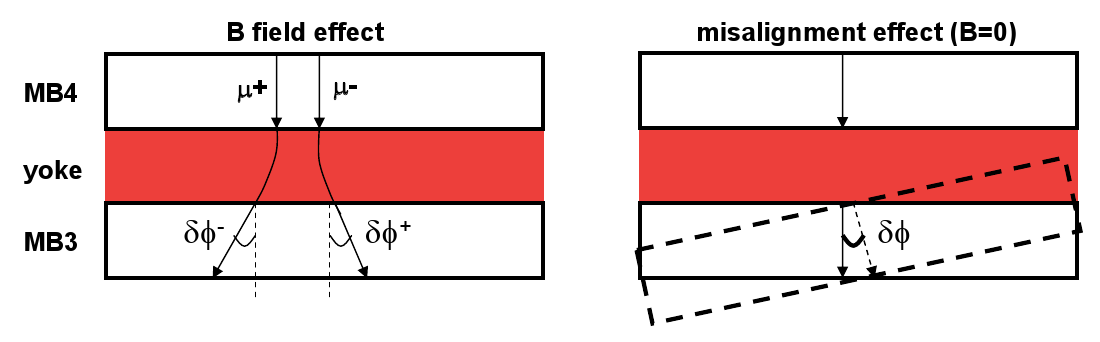
\includegraphics[width=\linewidth]{angular_diagram.png}

%% \vspace{1 cm}
%% \hfill 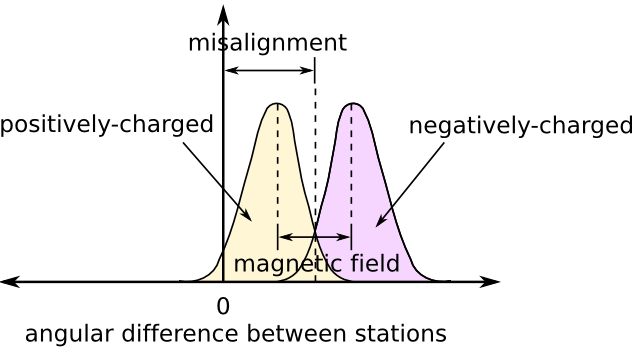
\includegraphics[width=0.75\linewidth]{angular_difference_plot.png}

%% \vspace{1 cm}
%% \end{columns}
%% \end{frame}

%% \begin{frame}
%% \frametitle{Sample $B_z$ measurements}
%% {\tiny Sara Bolognesi}

%% 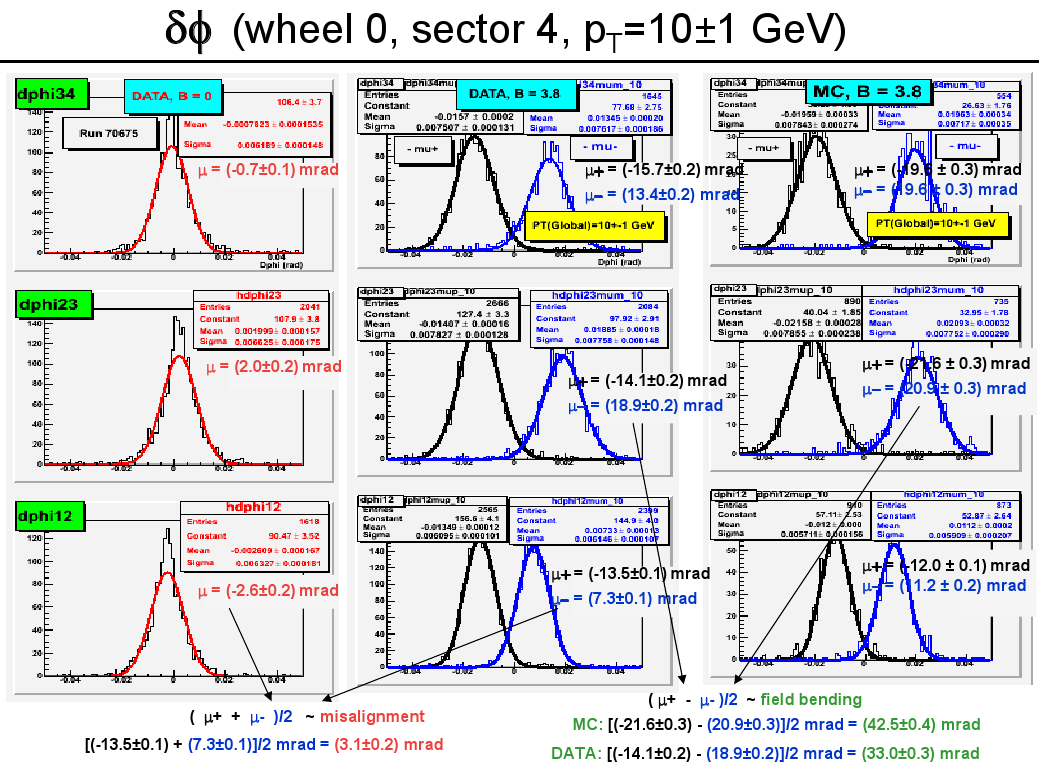
\includegraphics[width=\linewidth]{ugo_analysis.png}
%% \end{frame}

%% \begin{frame}
%% \frametitle{Summary of $B_z$ measurements}
%% \begin{columns}
%% \column{0.8\linewidth}
%% 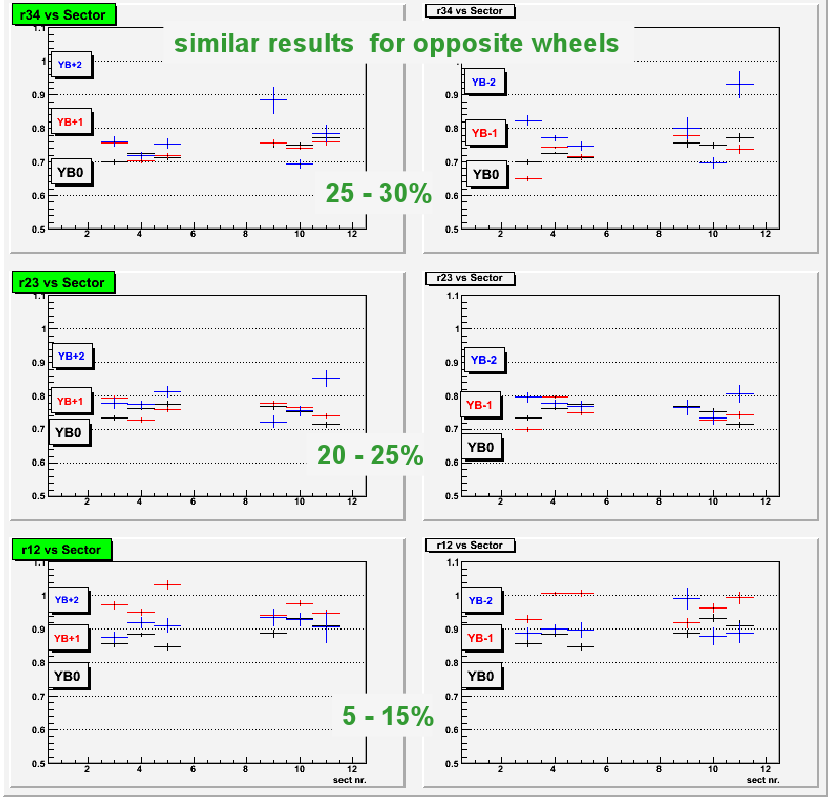
\includegraphics[width=\linewidth]{ugo_analysis2.png}

%% \column{0.3\linewidth}
%% {\tiny Sara Bolognesi} 

%% \vspace{1.25 cm}
%% $\left(B_z\big|_{\mbox{\scriptsize data}}\right) / \left(B_z\big|_{\mbox{\scriptsize MC}}\right)$

%% \vspace{0.5 cm}
%% \mbox{$10 < p_T < 50$~GeV\hspace{-1 cm}}

%% \vspace{0.5 cm}
%% Real $B_z$ is generally smaller than simulated

%% \vspace{3.25 cm}
%% \end{columns}
%% \end{frame}

%% \begin{frame}
%% \frametitle{Comparison with flux loops}

%% \begin{itemize}
%% \item ``data/MC'' is the fractional $B_z$ error determined by segments
%% \item The agreement is coarse at best
%% \end{itemize}

%% \vfill
%% 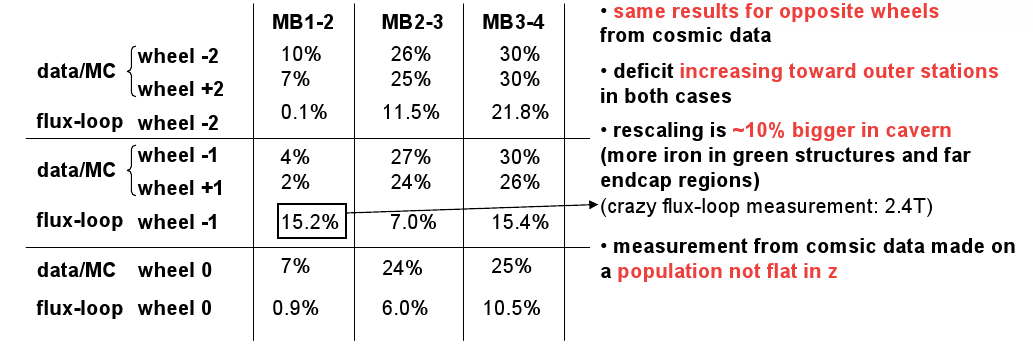
\includegraphics[width=\linewidth]{flux_loop_table.png}
%% \end{frame}

\begin{frame}
\frametitle{What about $B_r$ errors?}

\vspace{0.5 cm}
Inside of a DT drift cell:

\vspace{0.2 cm}
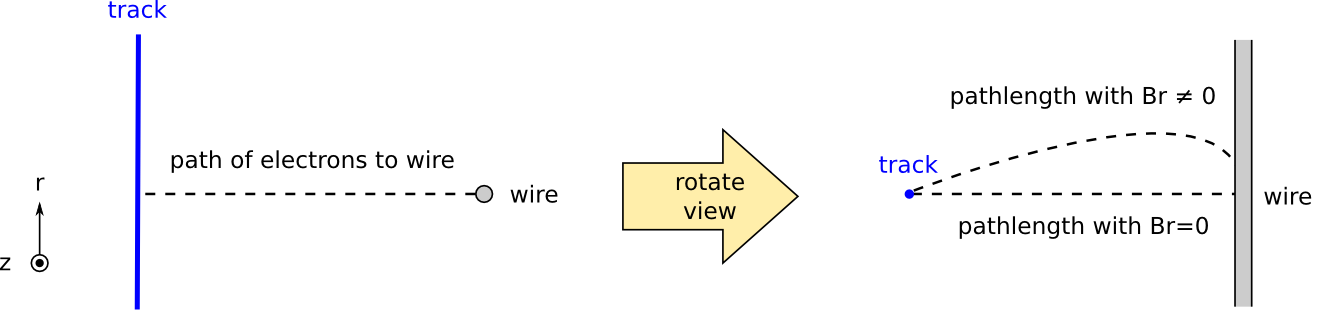
\includegraphics[width=\linewidth]{drift_explanation.png}

\vfill
\begin{itemize}
\item While muon momentum may be parallel with the radial direction,
  current of electrons drifting to wire is always perpendicular
\item Path is distorted by field, yielding a reduction in the
  apparent drift velocity (when computed as distance
  between track \mbox{and wire$/$drift time)\hspace{-1 cm}}
\item Variations in $v_{\mbox{\scriptsize drift}}$ are sensitive to
  $B_r$, including any error with respect to simulation
\item Independent of misalignment, though not a cross-check \\ (because this is $B_r$, not $B_z$)
\end{itemize}
\end{frame}

\begin{frame}
\frametitle{Qualitatively reproduces $B_r$ map}

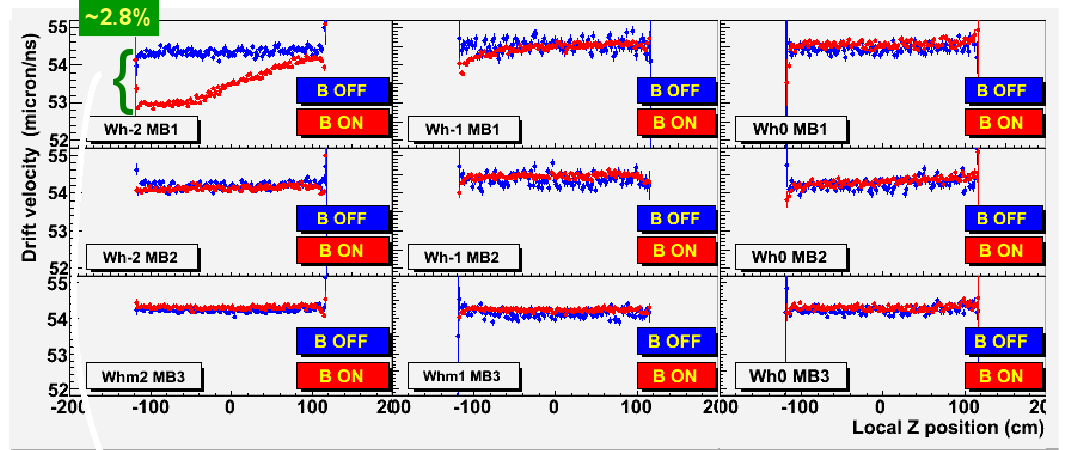
\includegraphics[width=0.95\linewidth]{cruz_analysis2.png}

\vfill
\begin{columns}
\column{0.5\linewidth}
Field map:

\vspace{0.2 cm}
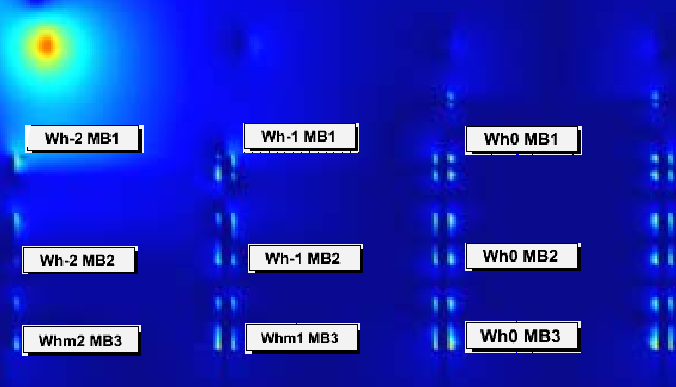
\includegraphics[width=\linewidth]{Br_simulation.png}

\column{0.5\linewidth}

Conversion to $B_r$ (test beam):

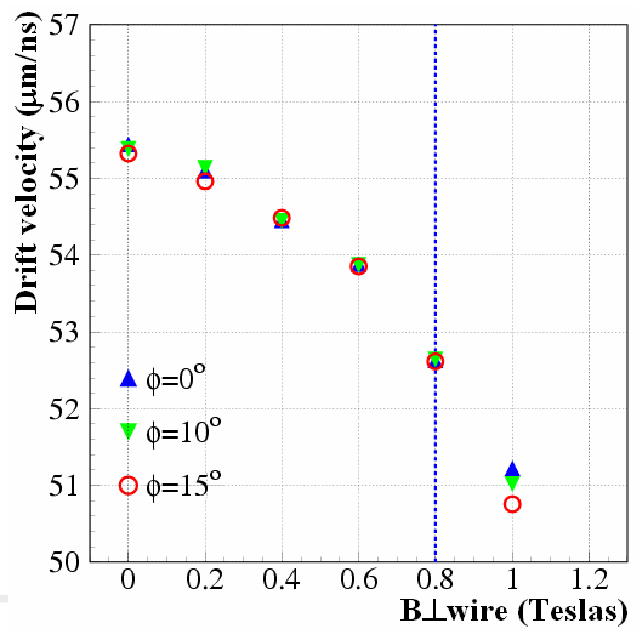
\includegraphics[width=0.65\linewidth]{cruz_analysis3.png} \hfill {\tiny Mary-Cruz Fouz}
\end{columns}
\end{frame}

\begin{frame}
\frametitle{$B_r$ is also smaller than simulation}
\framesubtitle{but only in high-field chambers}

\vspace{-0.25 cm}
\begin{center}
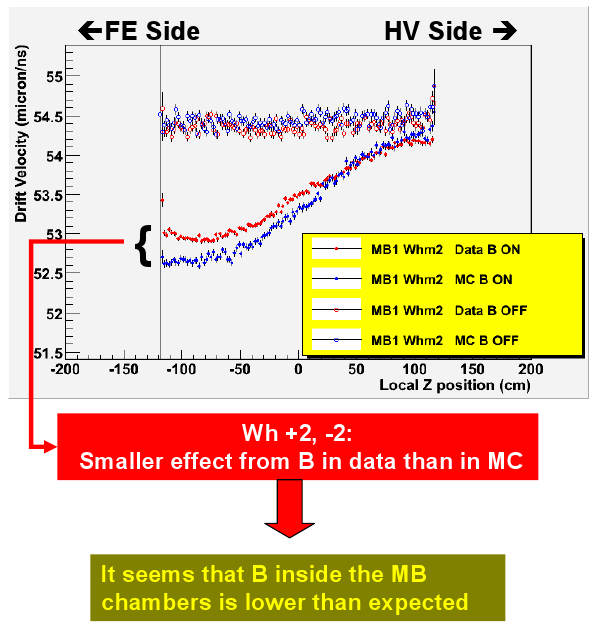
\includegraphics[width=0.7\linewidth]{cruz_analysis.png}
\end{center}

\vspace{-0.75 cm}
\hfill {\tiny Mary-Cruz Fouz}
\label{numpages}
\end{frame}

%% \begin{frame}
%% \frametitle{Initial $B_z$ analysis in the endcap}

%% \begin{itemize}
%% \item Compares $p_T$ of endcap stand-alone muons with tracker tracks
%% \item Sensitive to integral of $B_z$ error over path of tracks
%% \item Result: $B_z$ is about 10\% lower in data than in simulation \\ (assuming correct tracker momentum scale)
%% \item Work in progress!
%% \end{itemize}

%% \begin{center}
%% 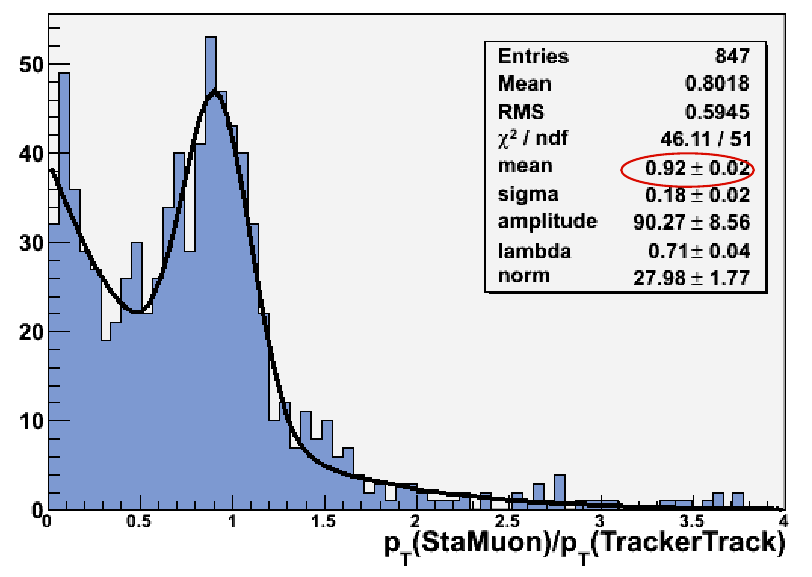
\includegraphics[width=0.7\linewidth]{endcap_result.png}
%% \end{center}

%% \vspace{-0.75 cm}
%% \hfill {\tiny Didar Dobur}
%% \end{frame}

%% \begin{frame}
%% \frametitle{Synthesis of measurements}

%% \begin{columns}
%% \column{0.5\linewidth}
%% \begin{center}
%% \textcolor{darkblue}{\Large $B_z$}
%% \end{center}

%% 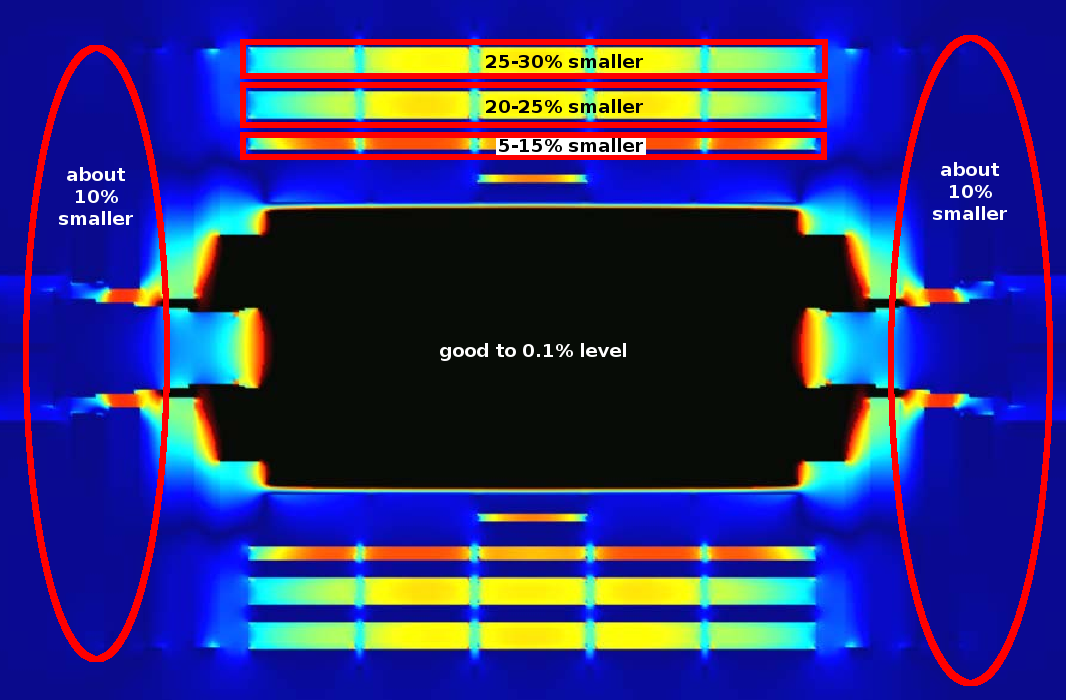
\includegraphics[width=\linewidth]{iguana_Bz.png}

%% \column{0.5\linewidth}
%% \begin{center}
%% \textcolor{darkblue}{\Large $B_r$}
%% \end{center}

%% 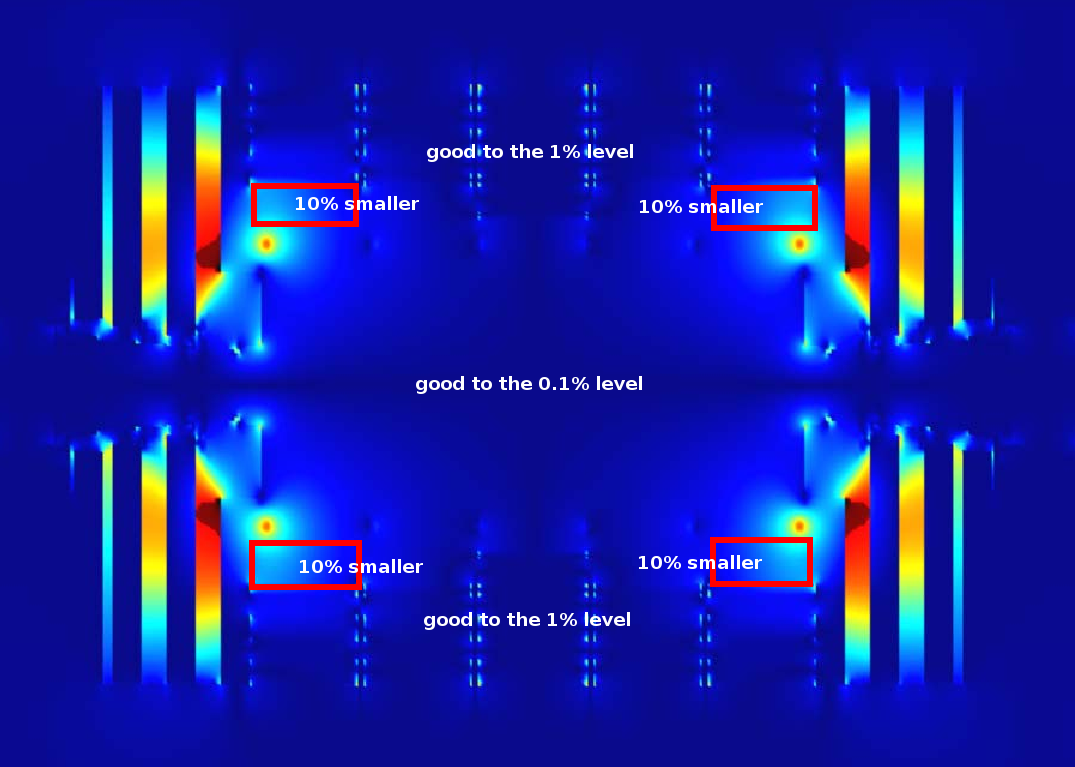
\includegraphics[width=\linewidth]{iguana_Br.png}
%% \end{columns}

%% \vfill
%% \begin{itemize}
%% \item If the field is at full strength in the tracker but smaller everywhere else, where are the field lines going?
%% \begin{itemize}
%% \item close to the beamline?  Maybe that explains the CASTOR \mbox{forces\ldots?\hspace{-1 cm}}
%% \end{itemize}

%% \item Ultimately, the field measurements must be understood in terms of an updated simulation
%% \end{itemize}
%% \end{frame}

%% \begin{frame}
%% \frametitle{What went wrong?}

%% \begin{columns}
%% \column{0.4\linewidth}
%% \begin{itemize}\setlength{\itemsep}{0.25 cm}
%% \item The magnetic field was simulated with CMS in isolation; no surrounding green structure as is in the cavern
%% \item Quick check: adding a conducting pillbox around CMS can overcorrect for the effect
%% \item Magnitude of corrections are therefore in the right ballpark
%% \item \mbox{Challenge will be to make the simulation more realistic\hspace{-5 cm}}
%% \end{itemize}

%% \column{0.6\linewidth}
%% \mbox{ } \hfill {\tiny Dietrich Liko}

%% \vspace{0.2 cm}
%% 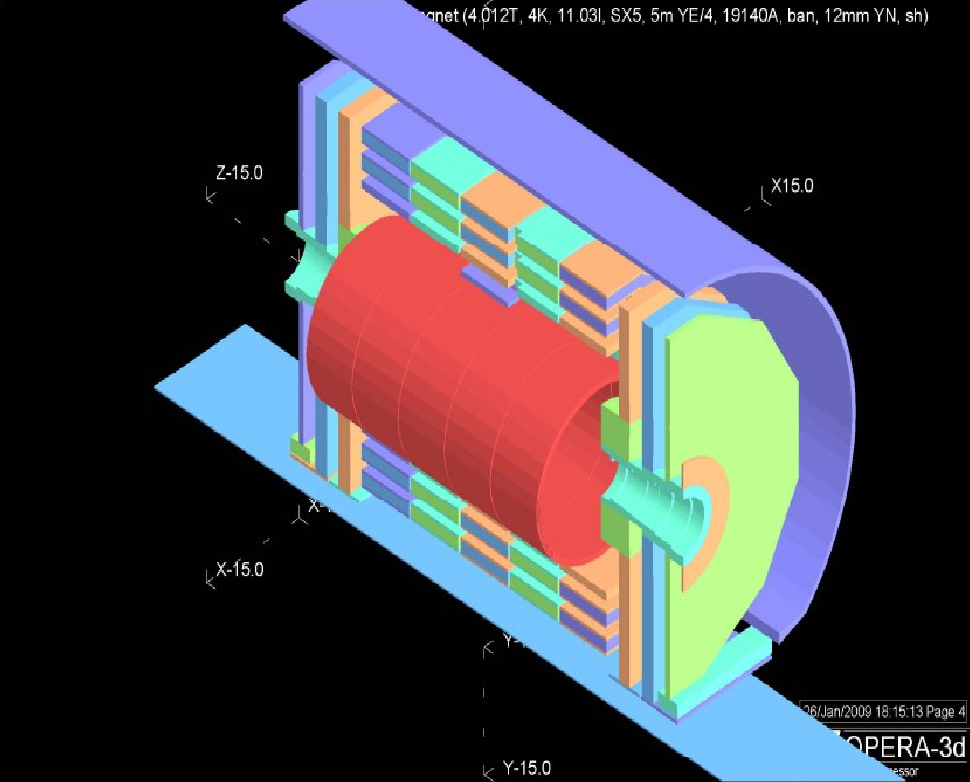
\includegraphics[width=\linewidth]{newsimulation.png}
%% \end{columns}
%% \end{frame}

%% %% \section*{First section}
%% %% \begin{frame}
%% %% \begin{center}
%% %% \Huge \textcolor{blue}{First section}
%% %% \end{center}
%% %% \end{frame}

%% \begin{frame}
%% \frametitle{Summary}
%% \begin{itemize}\setlength{\itemsep}{0.65 cm}
%% \item Muon tracking is far from perfect, but we're finding and
%%   correcting the kinds of distortions one might expect
%% \begin{itemize}
%% \item improvements to barrel alignment in second CRAFT re-processing
%% \item emerging picture of magnetic field map
%% \end{itemize}

%% \item Tracking datasets are rich: many problems that appear to be
%%   entangled can be cleanly decoupled by considering the right
%%   variables
%% \begin{itemize}
%% \item but comparisons with completely independent methods, such as the
%%   hardware alignment system and $\vec{B}$-field flux loops, is always
%%   helpful
%% \end{itemize}

%% \item CRAFT has been a productive shakedown cruise so far
%% \end{itemize}
%% \label{numpages}
%% \end{frame}

\end{document}
